\newpage
%%%%%%%%%%%%%%%%%%%%%%%%%%%%%%%%%%%%%%%%%%%%%%%%%%%%%%%%%%%%%%%%%%%%%%%%%%%%%%%%%%%%%%%%%%%%%%%%%%%%%%%%%%%%%%%%%%%%%%%%%%%%%%%%%%%%%%%%%%%%%%%%%%%%%%%%%%%%%%%%%%%%%%%
\chapter{Characterisation and estimation of the Standard Model backgrounds}
\label{sec:BackgroundEstimation}
After the application of the signal candidate selection, explained in the previous section, the background arising from Standard Model processes is dramatically reduced.
Only two events in the simulated \WJets sample remain.
One of these originates from an unreconstructed muon, the other one from an unreconstructed electron.
This implies, that the electron, muon, and tau vetos cannot reject all leptons because some are not properly reconstructed.
Due to the limited size of the simulated \WJets dataset (15 times smaller than the number of events expected from \WJets processes during 2012 data taking), 
it is not possible to rely on a full simulation-based estimation of the leptonic background.
The underlying mechanism of the non-reconstruction of a lepton and the corresponding methods to estimate the leptonic background will be explained in detail in Section~\ref{sec:LeptonicBkg}.

Furthermore, there is the possibility that a track is reconstructed out of a set of hits that do not origin from only one single particle.
Such tracks are called ``fake tracks''. 
Background tracks arising from a combination of unrelated hits will be explained in the following Section~\ref{sec:FakeBkg}.
It should be noted that the fake background is contributing through all SM processes, not only via \WJets.
Still, as the characteristics of fake tracks are independent of the underlying process, this background can also be studied on simulation using \WJets events only.
%The limited quality of the $dE/dx$ simulation enforces anyways a data-based background estimation method.



%%%%%%%%%%%%%%%%%%%%%%%%%%%%%%%%%%%%%%%%%%%%%%%%%%%%%%%%%%%%%%%%%%%%%%%%%%%%%%%%%%%%%%%%%%%%%%%%%%%%%%%%%%%%%%%%%%%%%%%%%%%%%%%%%%%%%%%%%%%%%%%%%%%%%%%%%%%%%%%%%%%%%%%
%%%%%%%%%%%%%%%%%%%%%%%%%%%%%%%%%%%%%%%%%%%%%%%%%%%%%%%%%%%%%%%%%%%%%%%%%%%%%%%%%%%%%%%%%%%%%%%%%%%%%%%%%%%%%%%%%%%%%%%%%%%%%%%%%%%%%%%%%%%%%%%%%%%%%%%%%%%%%%%%%%%%%%%
\section{Fake background}
\label{sec:FakeBkg}
Fake tracks are tracks that are not reconstructed out of the trajectory of one single particle.
The rate at which this wrong reconstruction occurs is highly restrained by the quality cuts on $\chi^2$ and the vertex compatibility of the track reconstruction algorithm.
Details on the reconstruction algorithm of tracks at CMS can be found in Section~\ref{FIXME}.

The probability of reconstructing a fake track is strongly correlated with the number of hits in the tracker system.
This can be seen in Fig.~\ref{fig:NValidFakes}, where the normalised distribution of the number of hits from fake tracks is depicted.
\begin{figure}[!b]
  \centering 
  \begin{tabular}{c}
    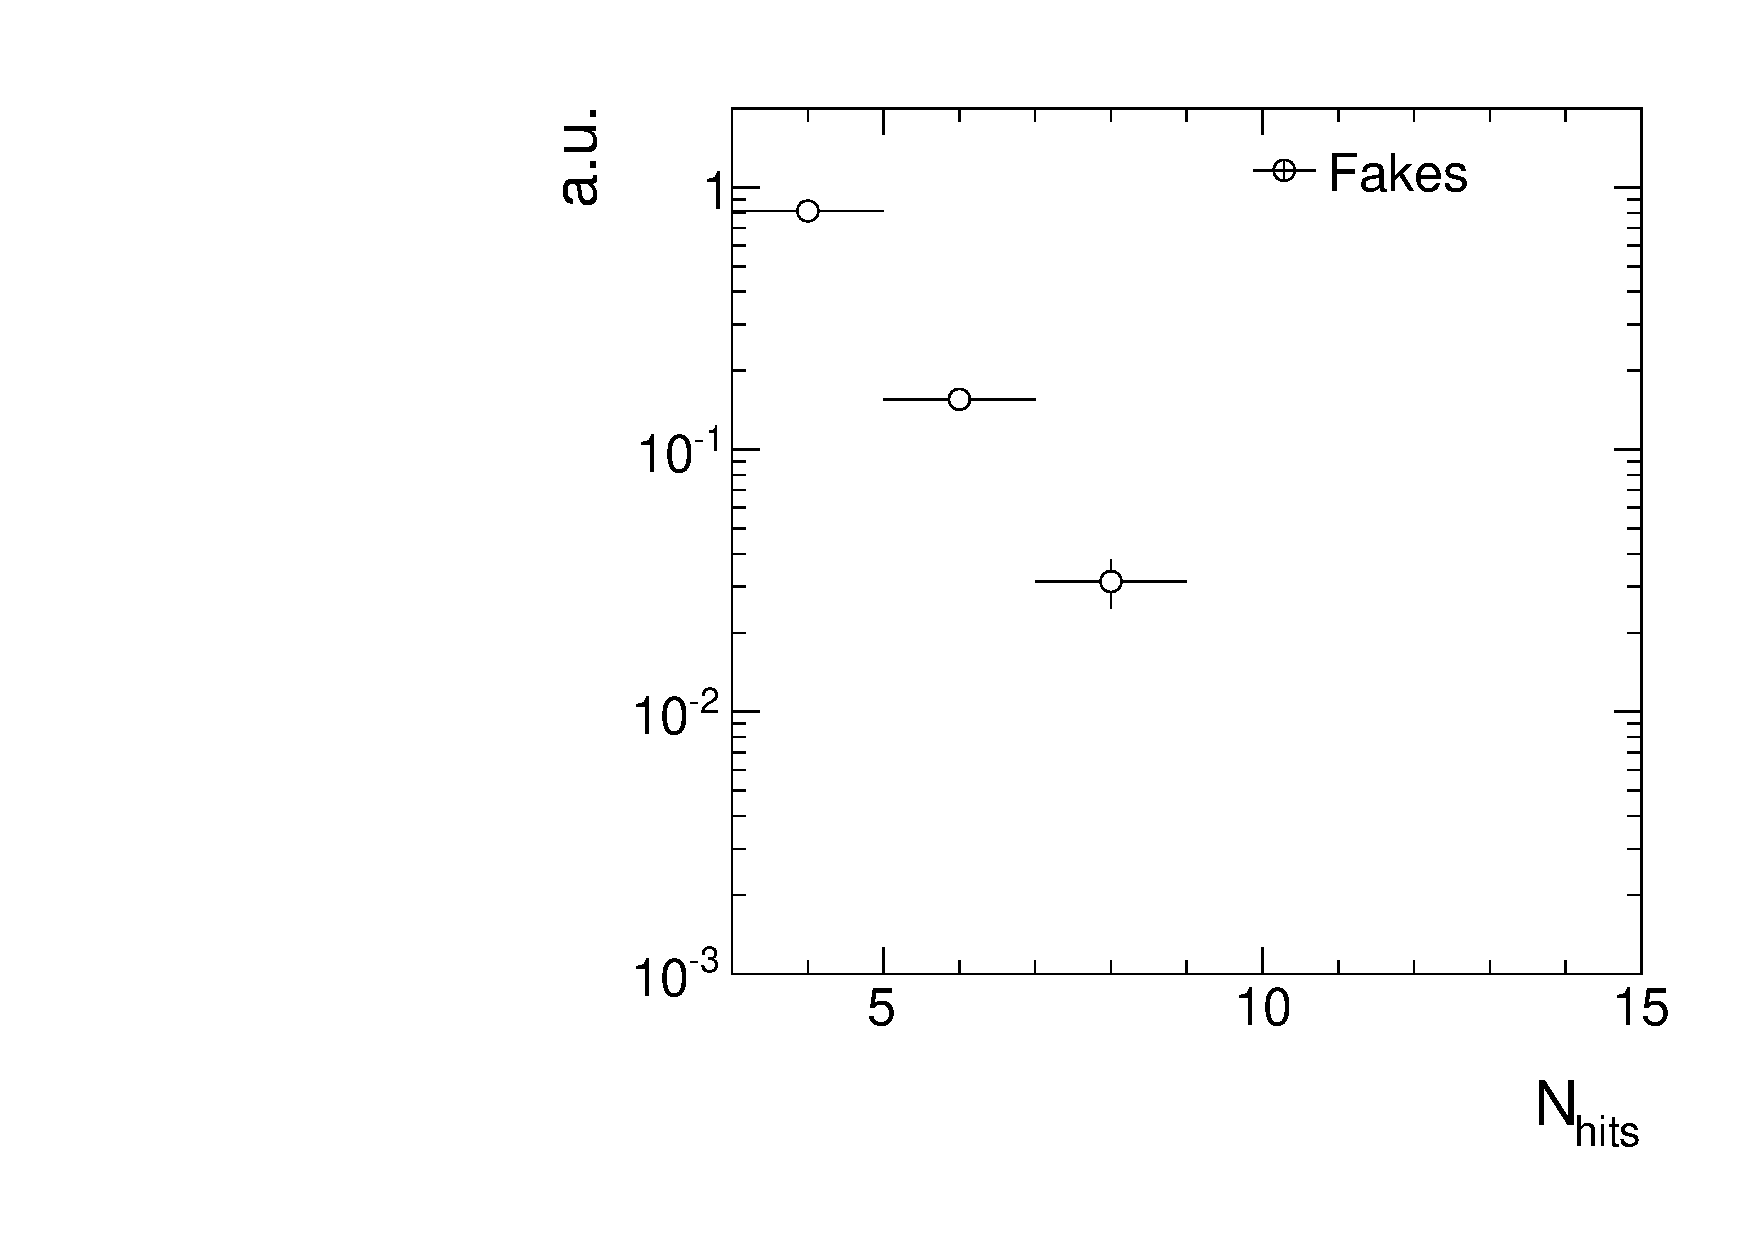
\includegraphics[width=0.49\textwidth]{figures/analysis/Background/NValidForFakes_chiTracksfullSelectionNoTriggerCuts.pdf}
  \end{tabular}
  \caption{Normalised distribution of the number of hits for fake tracks after the signal candidate selection from Table~\ref{tab:SummaryCuts}.
           To increase the statistical precision, only track selection requirements are applied.}
  \label{fig:NValidFakes}
\end{figure}
There are almost no fakes with a number of hits larger than seven.
In simulation, fake tracks are defined as tracks that cannot be matched to a generator-level particle within a distance of $\Delta R < 0.01$.

Fakes are efficiently suppressed by the requirements of no missing middle or inner hits and the compatibility with the primary vertex.
Unfortunately, wrongly reconstructed tracks which pass these criteria, do also easily pass the $\ecalo<5\gev$ requirement with high efficiency.\\

In this analysis, the estimation of the fake background is split into two parts.
First, the background is determined inclusively in \dedx.
Second, the \dedx (\ias) distribution is estimated with the help of a fake enriched control region. 
This second step is needed to enable an optimisation in \dedx (see Section~\ref{sec:Optimisation}).

\subsection*{Inclusive fake background estimation}
The inclusive background estimation closely follows the background estimation method done in~\cite{bib:CMS:DT_Thesis,bib:CMS:DT_8TeV_AN}.
It aims at determining the probability of having a fake track in an event that passes the full signal candidate selection (Table~\ref{tab:SummaryCuts}) plus a potential additional \pt selection cut that is determined in an
optimisation procedure (Section~\ref{sec:Optimisation}).
This probability will be called the fake rate \fakerate.

The inclusive fake background is estimated with the help of $Z\rightarrow\mu\bar{\mu}$ and $Z\rightarrow e\bar{e}$ events from data.
\Zlep events can be selected with high purity by requiring two well reconstructed muons or electrons that are opposite in charge and for which the invariant mass is around the $Z$-boson mass of $\sim90\gev$.
As these events do not contain further leptons from the hard interaction, any additional track is either an ISR jet, a soft particle from the underlying event or is a fake, reconstructed out of a combination of several soft particles.
Since the track-based signal candidate selection requires a track with a $\pt>20\gev$ that is no lepton or jet, it suppresses ISR jets and soft tracks from the underlying event.
Thus, applying the track-based signal candidate selection on \Zlep events selects fake tracks with high purity.


The selection of two well reconstructed muons and electrons is done with the single-muon and single-electron datasets listed in Table~\ref{tab:ElectronMuonCRDatasets}.
\renewcommand{\arraystretch}{1.5}
\begin{table}[!h]
\centering
\caption{Datasets used for the determination of the fake rate.}
\label{tab:ElectronMuonCRDatasets}
\makebox[0.99\textwidth]{
\begin{tabular}{lr}
\multicolumn{2}{c}{} \\
\toprule
Dataset  & Luminosity [\fbinv]   \\
\midrule
/SingleMu/Run2012A-22Jan2013-v1/AOD        &  0.876 \\
/SingleMu/Run2012B-22Jan2013-v1/AOD        &  4.405 \\
/SingleMu/Run2012C-22Jan2013-v1/AOD        &  7.040 \\
/SingleMu/Run2012D-22Jan2013-v1/AOD        &  7.369 \\ 
\midrule
/SingleElectron/Run2012A-22Jan2013-v1/AOD  &  0.876 \\
/SingleElectron/Run2012B-22Jan2013-v1/AOD  &  4.412 \\
/SingleElectron/Run2012C-22Jan2013-v1/AOD  &  7.050 \\
/SingleElectron/Run2012D-22Jan2013-v1/AOD  &  7.368 \\
\bottomrule
\multicolumn{2}{c}{} \\
\end{tabular}}
\end{table}  
For the $Z\rightarrow\mu\bar{\mu}$ selection an event is required to have two muons with $\pt>25\gev$ and $|\eta|<2.4$.
To suppress background from cosmic muons, the distance from the primary vertex must be less than $|d0|<0.2\cm$ in radial and $|dz|<0.5\cm$ in longitudinal direction.
In order to suppress background arising from jets that fake muons, various quality criteria are applied: it is required that there is at least one hit in the muon detector that is considered in the global muon fit, 
and that at least two measurements are from different muon detector stations.
Concerning the track of the muon in the tracker system, at minimum one hit in the pixel tracker and at least six hits in the full tracker system are required. 
An isolation criterion is applied that requires the sum of transverse momenta of all particle-flow particles in a cone of $\Delta R<0.4$ around the muon  to be less than 12\%.
Finally, the muons are required to be opposite in charge and to have an invariant mass between $80-100\gev$.
The $Z\rightarrow\mu\bar{\mu}\,+\,\text{fake track}$ selection is summarised in Table~\ref{tab:FakeMuonSample}.
\renewcommand{\arraystretch}{1.5}
\begin{table}[!h]
\centering
\caption{Event selection cuts for the $Z\rightarrow\mu\bar{\mu}\,+\,\text{fake}$ control sample to estimate the inclusive fake background.}
\label{tab:FakeMuonSample}
\makebox[0.99\textwidth]{
\begin{tabular}{l|l l }
\multicolumn{3}{c}{} \\
\toprule
\multirow{12}{*}{\makecell[l]{Event-based \\ selection}}       &  Two global muons with & $\pt>25\gev$ \\
                                                               &                        & $|\eta|<2.4$ \\
                                                               &                        & $\sum\limits_{\Delta R<0.4} \pt^{\text{PF particle}}/\pt(\mu)<0.12$ \\
                                                               &                        & $\left.\frac{\chi^2}{ndof}\right\rvert_{\text{global track}}<10$ \\
                                                               &                        & $|d0|<0.2\cm$  \\
                                                               &                        & $|dz|<0.5\cm$  \\
                                                               &                        & \makecell[l]{$\geq$ 1 hit in the muon detector\\ \hspace{0.3cm} considered in global fit}  \\
                                                               &                        & $\geq$ 2 hits in different muon stations \\
                                                               &                        & $\geq$ 1 hit in the pixel detector  \\
                                                               &                        & $\geq$ 6 hits in the tracker system  \\
                                                               &  \multicolumn{2}{l}{Muons opposite in charge}                                     \\
                                                               &  \multicolumn{2}{l}{$80\gev<M_{\text{inv}}\left(\mu_1,\mu_2  \right)<100\gev$}        \\

\midrule

\multirow{4}{*}{\makecell[l]{Candidate track\\ selection}}    &  Good quality selection \\
                                                              &  Kinematic selection    \\
                                                              &  Lepton/jet veto        \\   
                                                              &  Isolation selection    \\  
\bottomrule
\multicolumn{3}{c}{} \\
\end{tabular}}
\end{table}

In order to select $Z\rightarrow e\bar{e}$ events in data, the two electrons are required to have \mbox{$\pt>25\gev$}, $|\eta|<2.5$ and no missing hits in the inner layers of the tracker.
Furthermore, the electrons need to pass a conversion veto as described in~\cite{bib:CMS:ConversionVeto_PAS} in order to reduce background arising from photon conversions.
An isolation requirement similar to the muon isolation criterion is applied with an increased threshold of 15\%.
The electron identification is further based on a multivariate technique developed within~\cite{bib:CMS:ElectronMVA} that exploits electron characteristics about the track quality, the ECAL cluster shapes, and the combination 
of the measurements in the tracker and in the ECAL.
Again, the two electrons must be opposite in charge and their invariant mass must be between $80-100\gev$.
A summary of the $Z\rightarrow e\bar{e}\,+\,\text{fake track}$ event selection can be found in Table~\ref{tab:FakeElectronSample}.\\
\renewcommand{\arraystretch}{1.5}
\begin{table}[!h]
\centering
\caption{Event selection cuts for the $Z\rightarrow e\bar{e}\,+\,\text{fake}$ control sample to estimate the inclusive fake background.}
\label{tab:FakeElectronSample}
\makebox[0.99\textwidth]{
\begin{tabular}{l|l l }
\multicolumn{3}{c}{} \\
\toprule
\multirow{8}{*}{\makecell[l]{Event-based \\ selection}}        &  Two Electrons with    & $\pt>25\gev$ \\
                                                               &                        & $|\eta|<2.5$ \\
                                                               &                        & $\sum\limits_{\Delta R<0.4} \pt^{\text{PF particle}}/\pt(e)<0.15$ \\
                                                               &                        & pass conversion veto~\cite{bib:CMS:ConversionVeto_PAS}    \\
                                                               &                        & no missing inner tracker hits\\
                                                               &                        & good MVA electron as defined in \cite{bib:CMS:ElectronMVA}  \\
                                                               &  \multicolumn{2}{l}{Electrons opposite in charge}                                     \\
                                                               &  \multicolumn{2}{l}{$80\gev<M_{\text{inv}}\left(e_1,e_2  \right)<100\gev$}        \\

\midrule

\multirow{4}{*}{\makecell[l]{Candidate track\\ selection}}    &  Good quality selection \\
                                                              &  Kinematic selection    \\
                                                              &  Lepton/jet veto        \\   
                                                              &  Isolation selection    \\  
\bottomrule
\multicolumn{3}{c}{} \\
\end{tabular}}
\end{table}  

When applying a \Zlep selection plus the candidate track selection, the selected track should be a fake.
If this is indeed the case can be tested on simulated \Zlep events.
As can be seen in Fig.~\ref{fig:BkgComposition}, a reasonable purity in fake tracks can be achieved by applying the candidate track selection on top of the \Zlep selection.
\begin{figure}[!b]
  \centering 
  \begin{tabular}{c}
    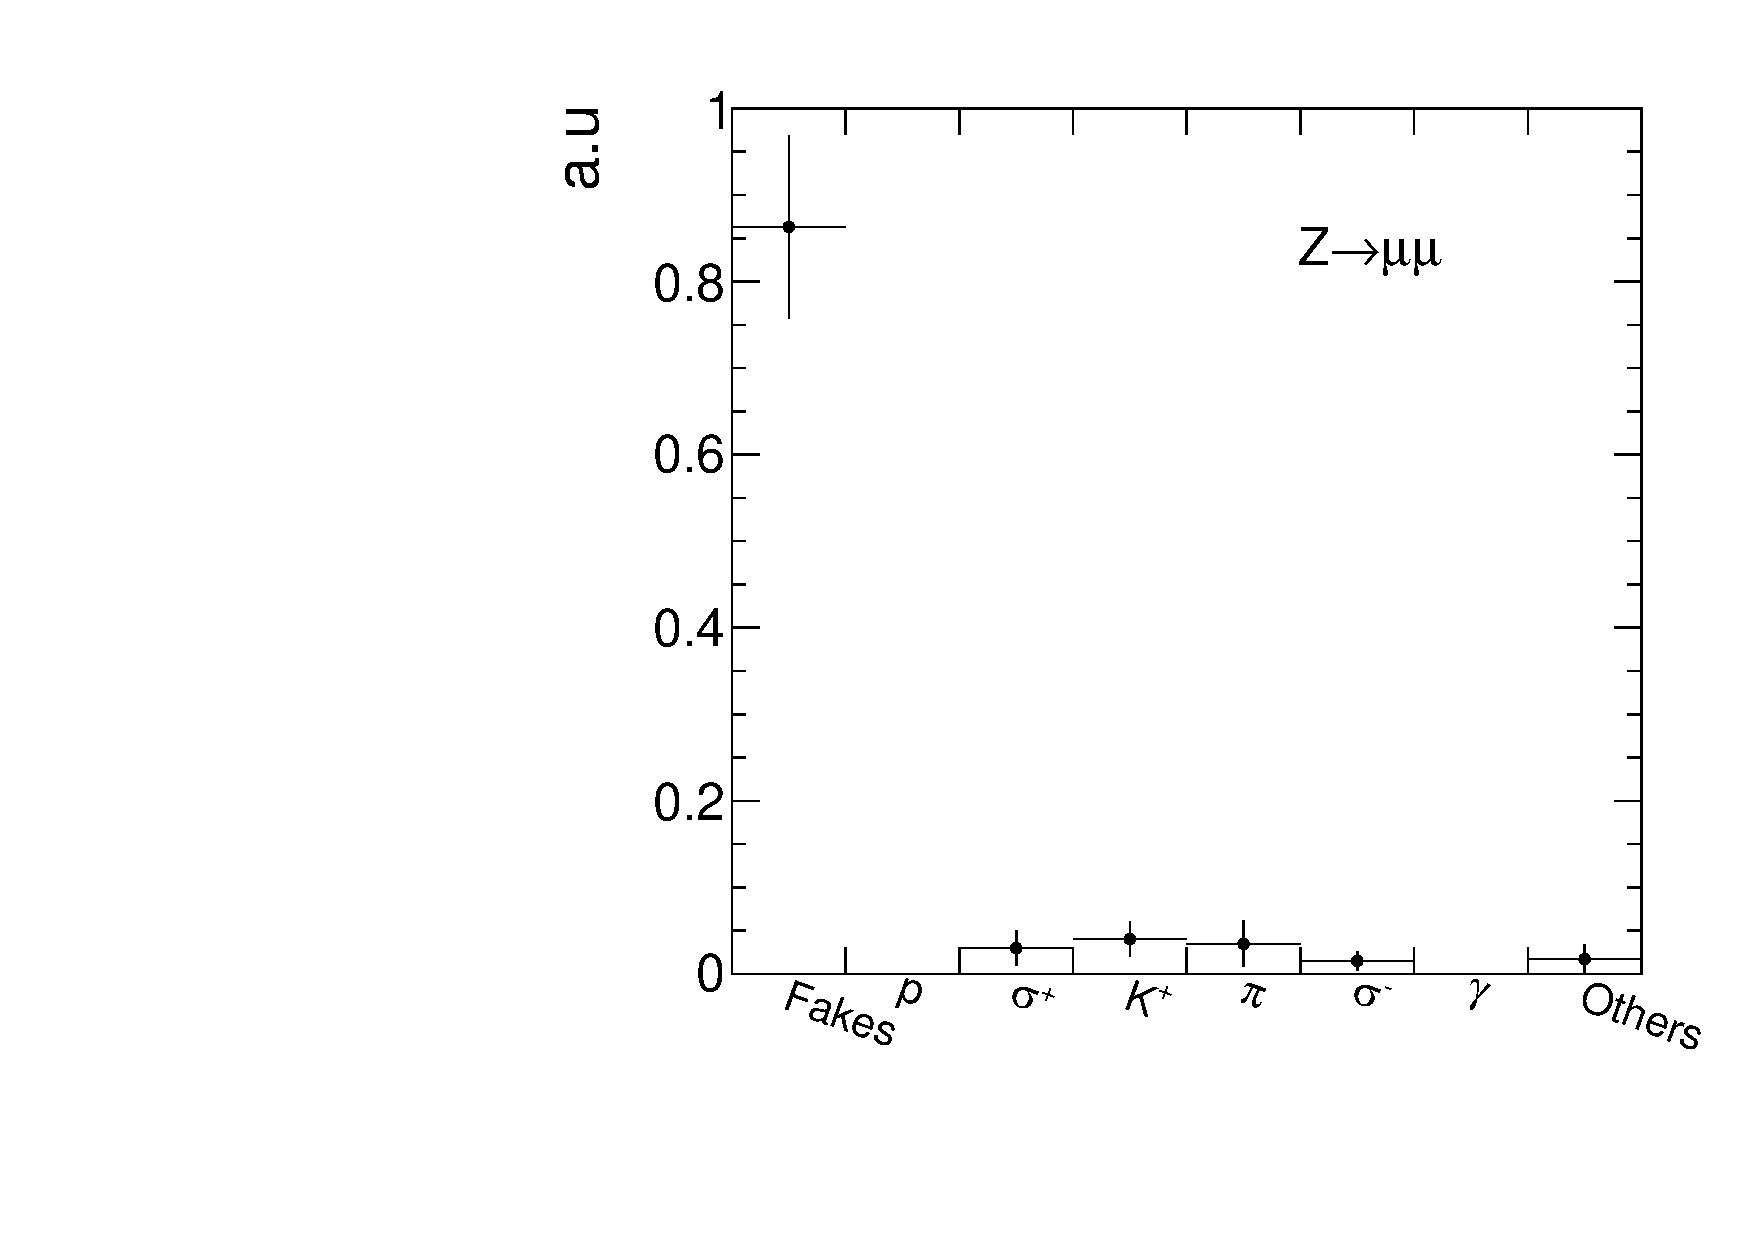
\includegraphics[width=0.49\textwidth]{figures/analysis/Background/ParticleCompositionInFakeCS_Mu.pdf}
    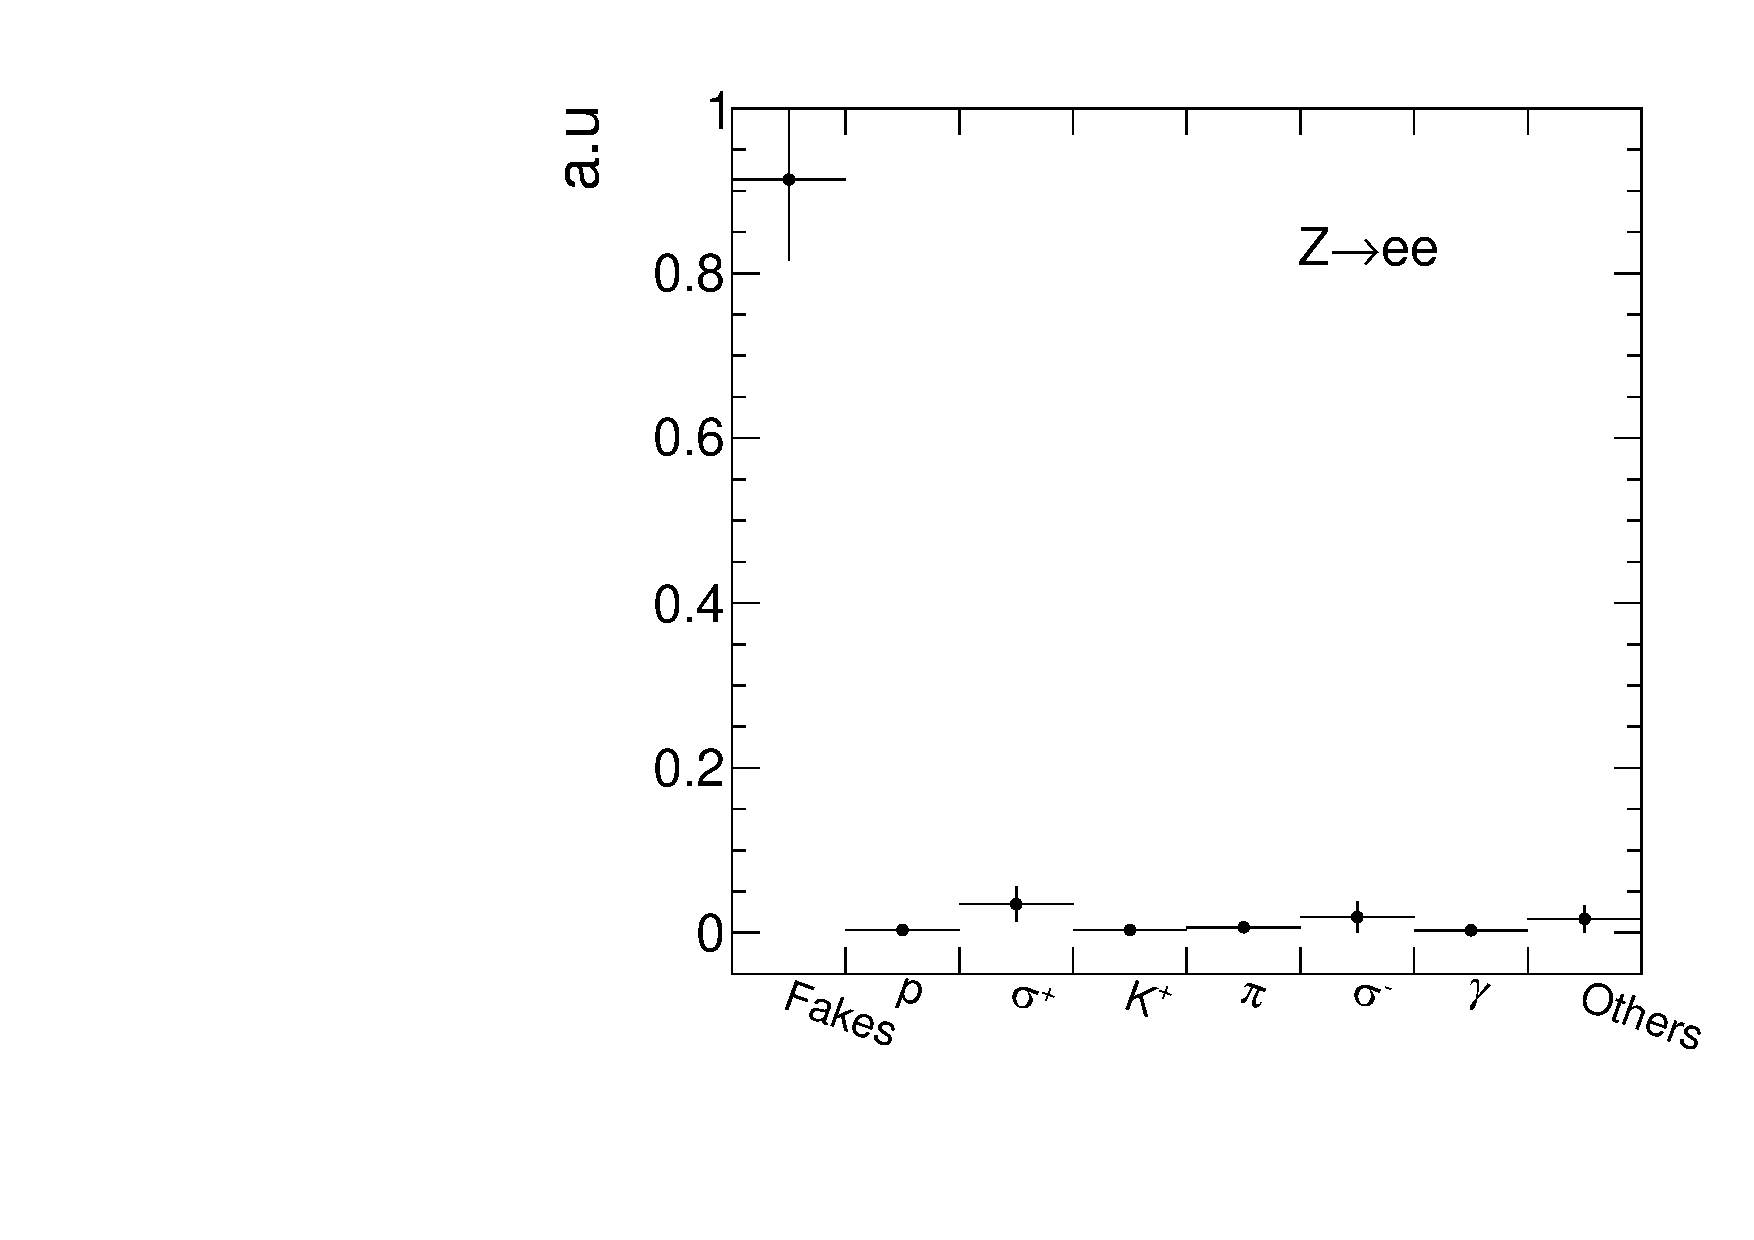
\includegraphics[width=0.49\textwidth]{figures/analysis/Background/ParticleCompositionInFakeCS_Ele.pdf}
  \end{tabular}
  \caption{Corresponding generator-level particles of all tracks within $Z\rightarrow \ell \bar{\ell}\,+\,\text{fake}$ that were selected according to the candidate track selection. 
           The full selection for tracks in $Z\rightarrow \mu \bar{\mu}$ events (left) is given in Table~\ref{tab:FakeMuonSample}.
           The full selection for tracks in $Z\rightarrow e \bar{e}$ events (right) is given in Table~\ref{tab:FakeElectronSample}.
           ``Fake'' means that no corresponding generator-level particle is found. }
  \label{fig:BkgComposition}
\vspace{50pt}
\end{figure}
In simulated $Z\rightarrow\mu\bar{\mu}$ events, a purity of 88\%, whereas in simulated $Z\rightarrow e\bar{e}$ events a purity of 92\% of fake tracks can be achieved.


As already mentioned, the fake rate is defined as the probability that an event contains a fake track that fulfils the candidate track selection.
Thus, for the \Zlep datasets it is defined as the number of events passing the full selection described in Table~\ref{tab:FakeMuonSample} (Table~\ref{tab:FakeElectronSample}) divided by the number of events that pass only the event-based selection in Table~\ref{tab:FakeMuonSample} (Table~\ref{tab:FakeElectronSample})
\begin{equation*}
\fakerate = \frac{N_{Z\rightarrow ll}^{\text{cand trk selection}}}{N_{Z\rightarrow ll}}
\end{equation*}
Fake rates are determined independently for the $Z\rightarrow \mu\bar{\mu}\,+\,\text{fake}$ and $Z\rightarrow e\bar{e}\,+\,\text{fake}$ event selection and then averaged to obtain the final fake rate. 
The fake rate with the candidate track selection given in Table~\ref{tab:SummaryCuts} is $\left( 6.86 \pm 0.25 \right) \cdot 10^{-5}$. 
This is not the final result as the optimisation in \pt will add an additional \pt selection cut to the candidate track selection.

Within~\cite{bib:CMS:DT_Thesis,bib:CMS:DT_8TeV_AN}, it was checked that the fake rate is constant for different processes.
This is shown in Fig.~\ref{fig:FakeRate} where the fake rate is depicted for the most important SM processes.
\begin{figure}[!b]
  \centering 
  \begin{tabular}{c}
    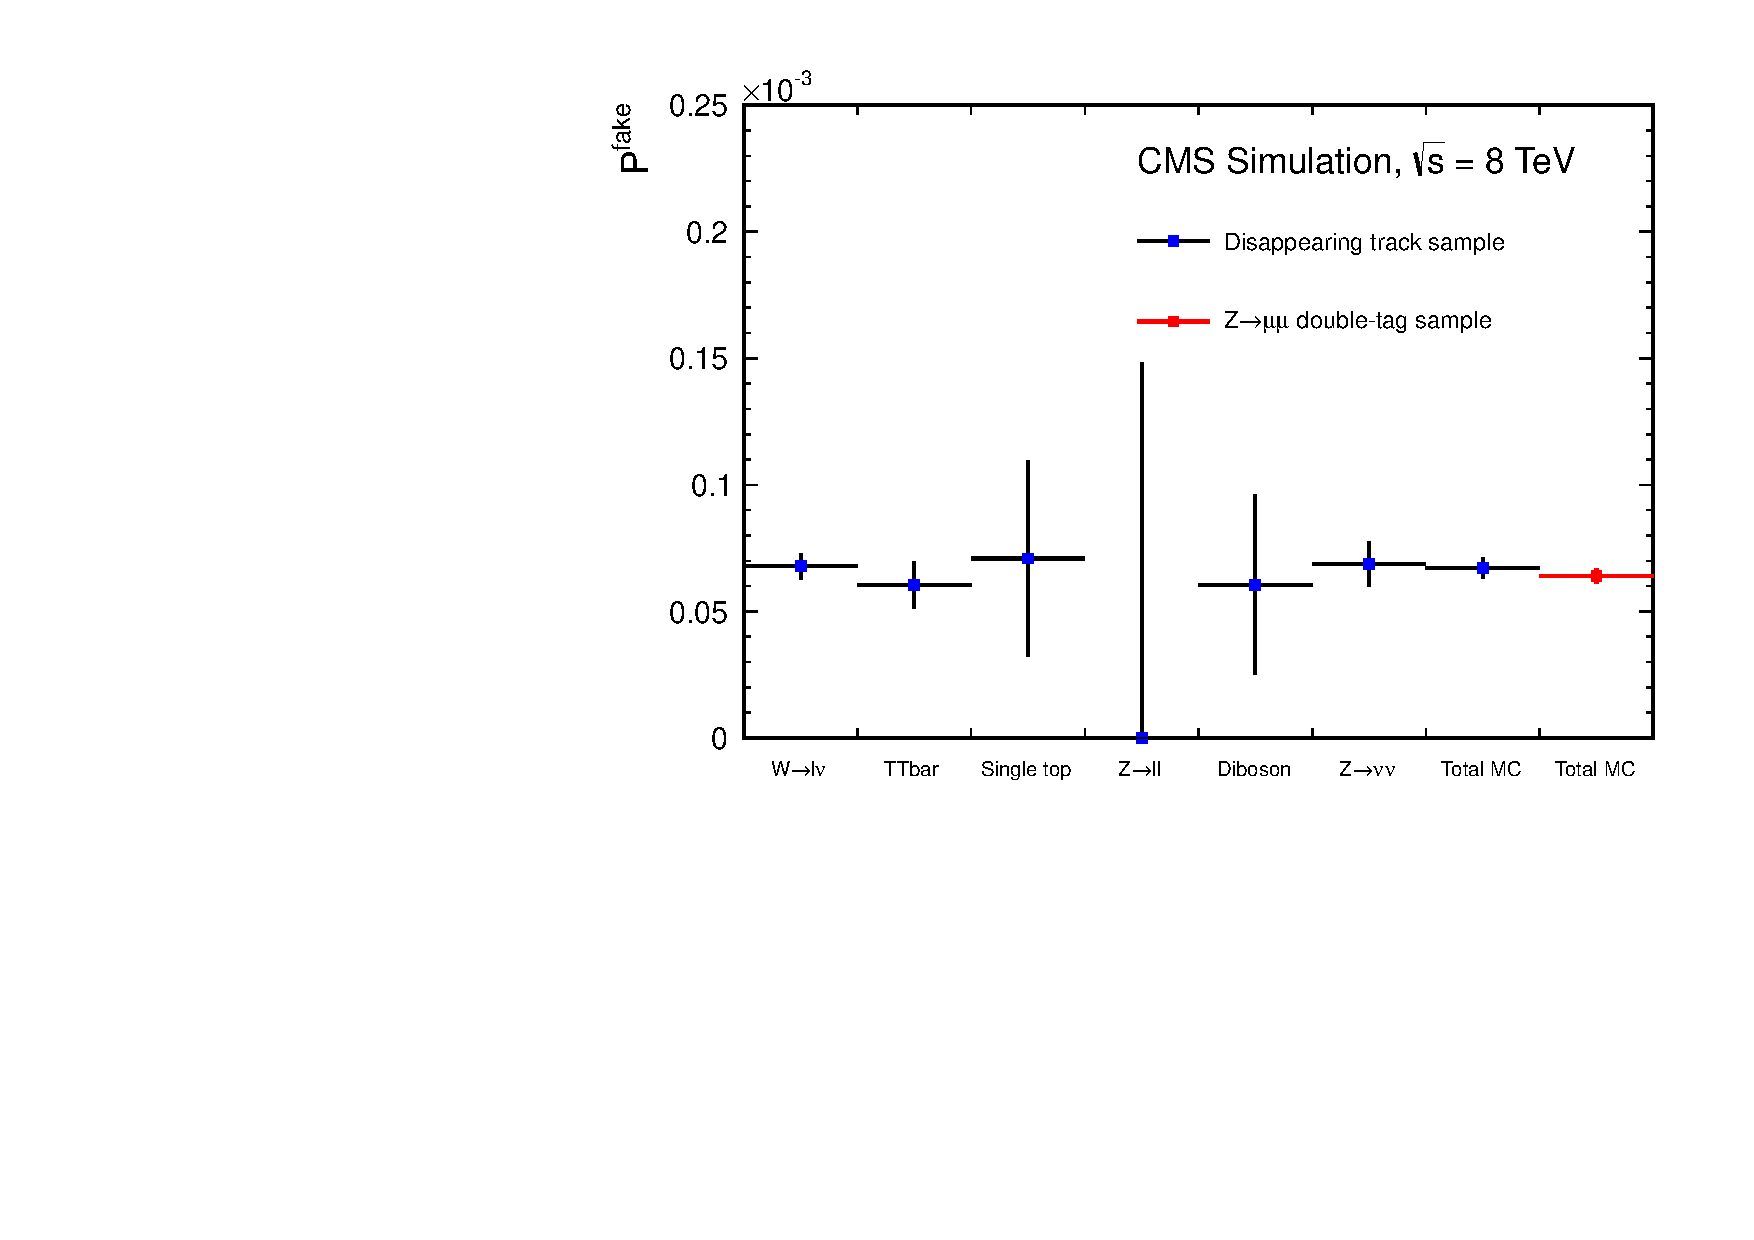
\includegraphics[width=0.79\textwidth]{figures/analysis/Background/fakeTrkRates.pdf}
  \end{tabular}
  \caption{Fake track rate estimated in \cite{bib:CMS:DT_Thesis,bib:CMS:DT_8TeV_AN} for tracks with four hits. Taken from \cite{bib:CMS:DT_8TeV_AN} }
  \label{fig:FakeRate}
\end{figure}
Since the fake rate is constant for different SM processes, the fake rate determined on the \Zlep dataset can be generalised for all SM background possibly contributing to this search.
Thus, the inclusive fake background can be estimated by multiplying the fake rate with the number of events selected from the MET dataset (Table ~\ref{tab:SearchSamples}) by applying the event-based signal candidate requirements from Table~\ref{tab:SummaryCuts}.
\begin{equation*}
N^{\text{fake, inclusive in I$_{\text{as}}$}}_{\text{bkg}} = \fakerate \cdot N_{\text{event-based selection}}^{\text{MET}}.
\end{equation*}
Given the number of events after the event-based selection of $N_{\text{event-based selection}}^{\text{MET}} = 1.38\cdot10^6$ and the fake rate cited above, 
the inclusive fake background can be estimated to $94.7\pm3.4$ for the candidate track selection.

It should be noted again that the inclusive fake background estimation will be only inclusive in \ias not in \pt.
That means that after the definition of the signal region, $N^{\text{fake, inclusive in I$_{\text{as}}$}}_{\text{bkg}}$ is determined with the additional optimal \pt selection.

Possible differences between the fake rate in \Zlep events and other SM processes are estimated on simulated events and taken into account as a systematic uncertainty (see Section~\ref{sec:FakeRateUncertainty}).

%%%%%%%%%%%%%%%%%%%%%%%%%%%%%%%%%%%%%%%%%%%%%%%%%%%%%%%%%%%%%%%%%%%%%%%%%%%%%%%%%%%%%%%%%%%%%%%%%%%%%%%%%%%%%%%%%%%%%%%%%%%%%%%%%%%%%%%%%%%%%%%%%%%%%%%%%%%%%%%%%%%%%%%
\subsection*{dE/dx shape of fake background}
The information about the energy release per path length for fake tracks should not be taken from simulated samples as the simulation of $dE/dx$ is not reliable (cf. Fig.~\ref{fig:Data-MC-Dedx_MIPs}).
Within this analysis the Asymmetric Smirnov discriminator \ias is used to discriminate signal against background with respect to \dedx (see Section~\ref{sec:Ias}). 
In order to estimate the \ias shape of fake tracks, a control region \fakeCR is defined that is enriched with fakes and shows the same \ias distribution as fake tracks in the signal region.

To enrich fake tracks, it is possible to invert the selection cuts on the number of missing middle and inner hits, \ie requiring at least one missing inner or middle hit $\left( N_{\text{miss}}^{\text{inner}} +N_{\text{miss}}^{\text{middle}}>0\right)$.
Figure~\ref{fig:NMissInnerAndMiddle} shows the distribution of the number of missing inner plus missing middle hits for fake and leptonic tracks in simulated \WJets events.
It can be seen that the enrichment of fakes by this selection works.
The resulting purity of fakes in \fakeCR is about 98\% (see Fig.~\ref{fig:IasSRCRFakes}). 
\begin{figure}[!b]
  \centering 
  \begin{tabular}{c}
    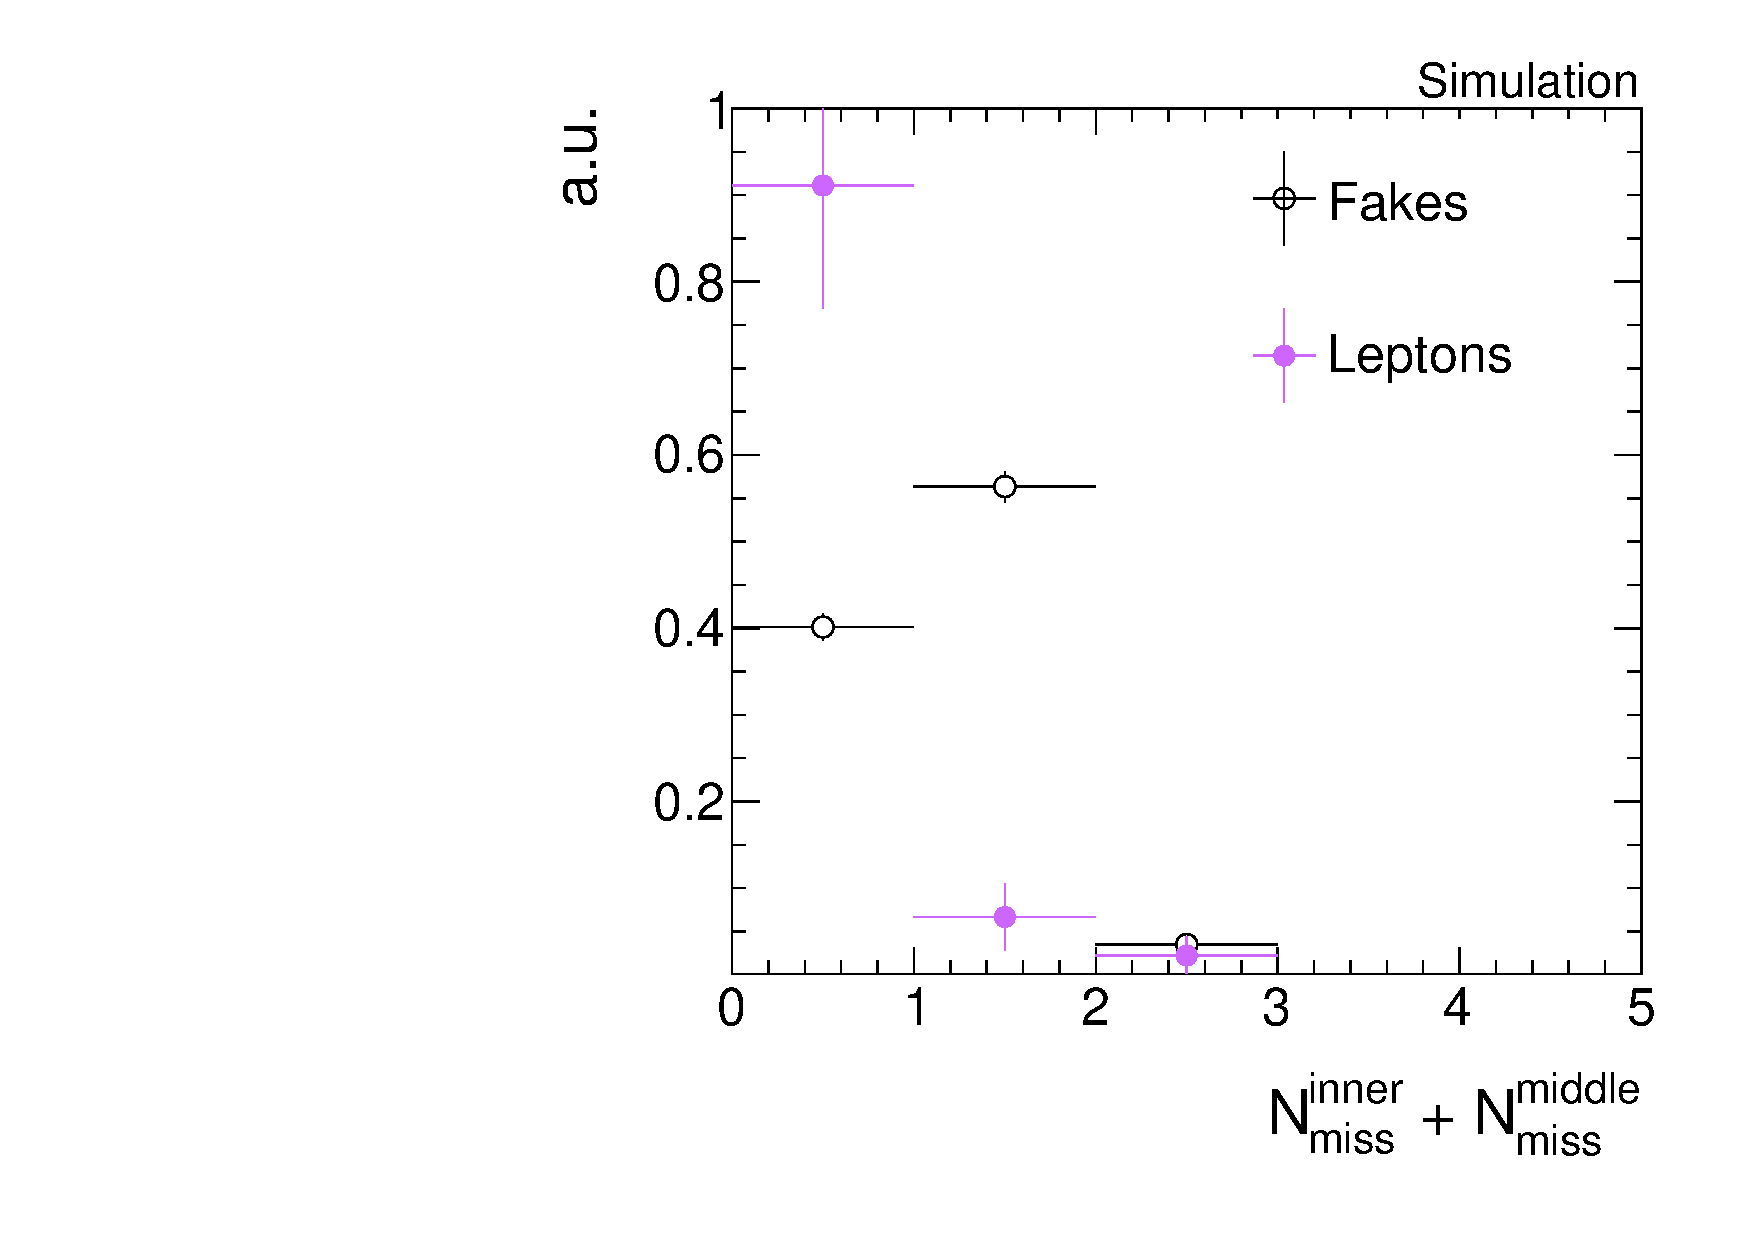
\includegraphics[width=0.49\textwidth]{figures/analysis/Background/NLostInnerPlusMiddleForAllBkg_chiTracksQCDsupressionTrigger.pdf}
  \end{tabular}
  \caption{Normalised number of missing inner plus missing middle hits for fake and leptonic tracks for the full candidate track selection with the selection requirements on $N_{\text{miss}}^{\text{inner}}$ and $N_{\text{miss}}^{\text{middle}}$ removed. Trigger requirements and QCD suppression cuts were removed to enhance the statistical precision.}
  \label{fig:NMissInnerAndMiddle}
\end{figure}

Additionally, it must be checked whether the \ias shape in \fakeCR is comparable to the \ias shape in the signal region.
As the exact definition of the signal region will be addressed during optimisation, this test is done for various \pt selection cuts.

The comparison of the \ias shape of fake tracks can only be done on simulation.
Thus, simulated \WJets events are used to select fake tracks in both regions.
A comparison of the shape for the candidate track selection and the \fakeCR is shown in Fig.~\ref{fig:IasSRCRFakes}.

\begin{figure}[!t]
  \centering 
  \begin{tabular}{c}
    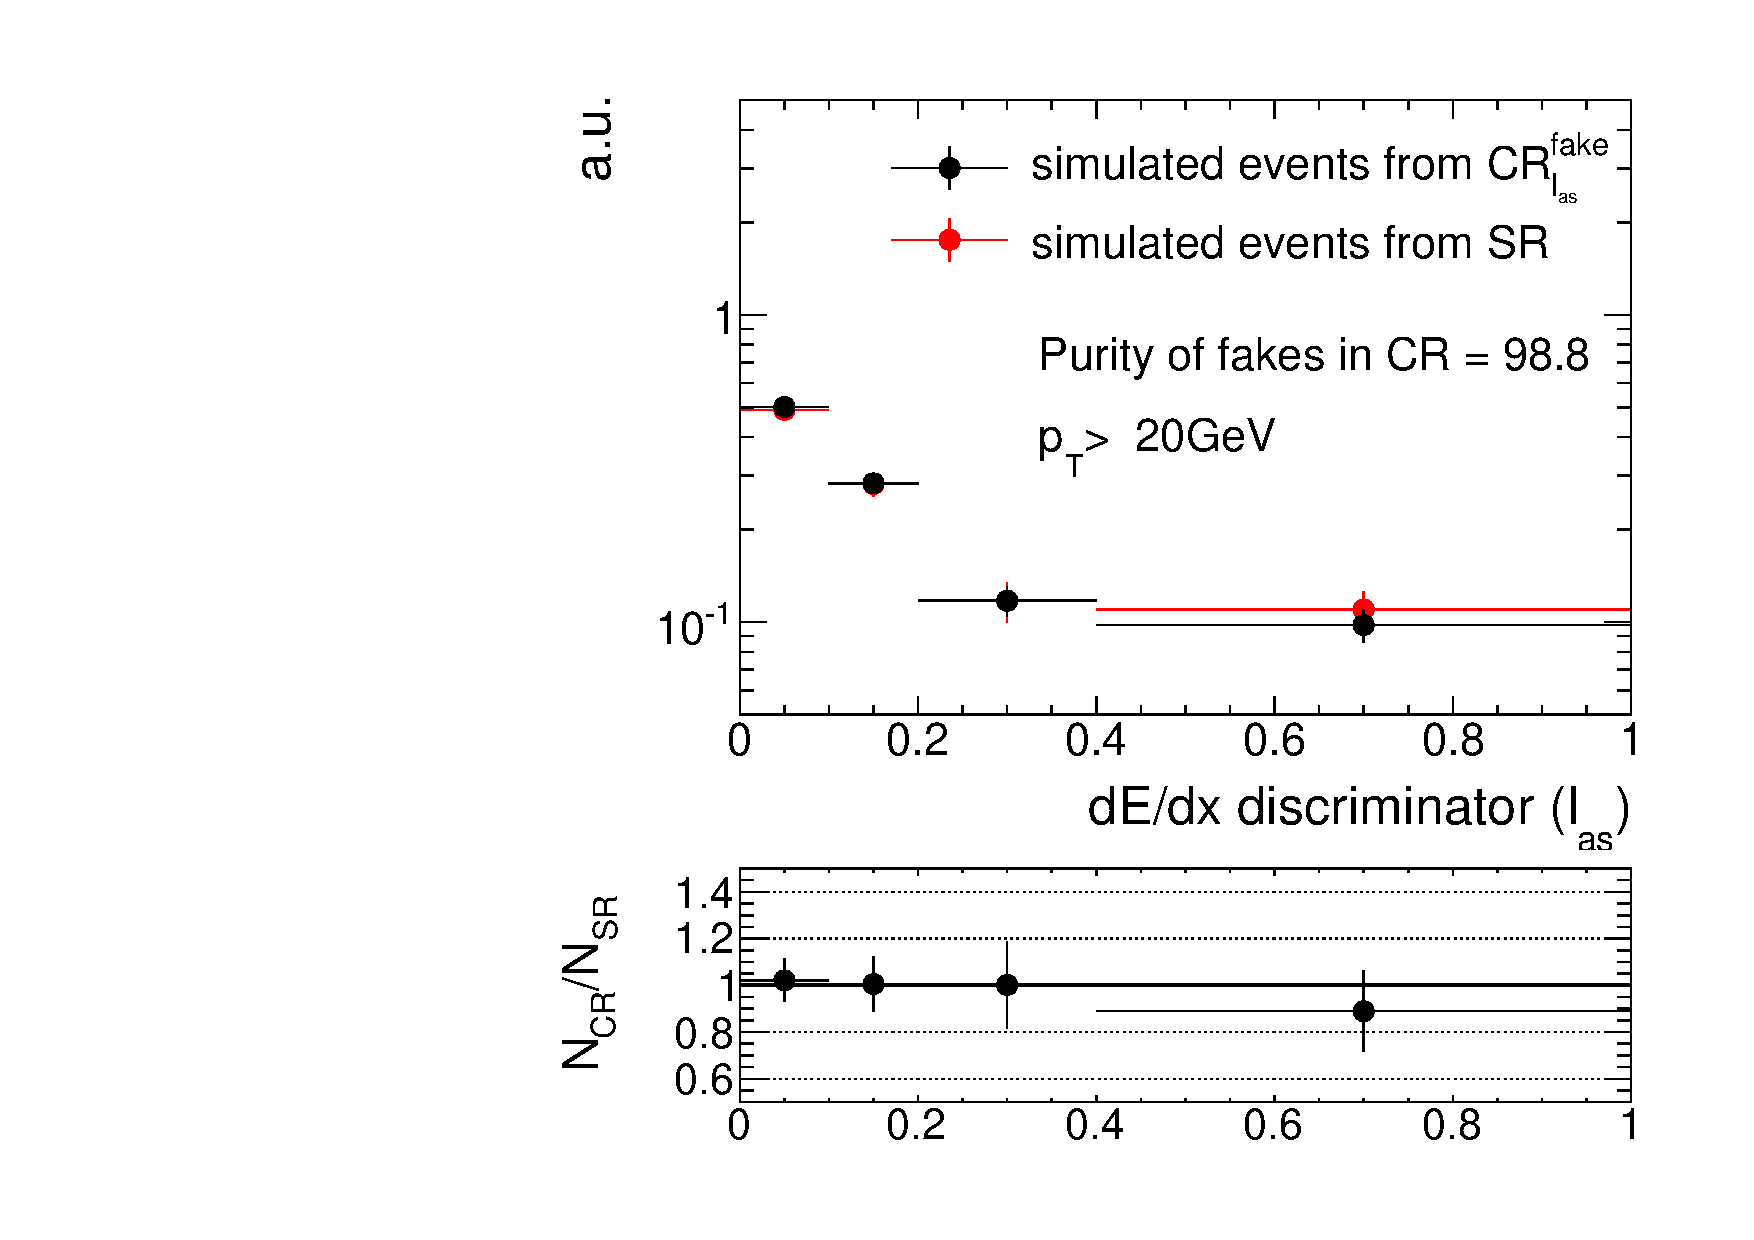
\includegraphics[width=0.49\textwidth]{figures/analysis/Background/hASmi_fakes_ECalaoLe5_trackPtGt20.pdf}
    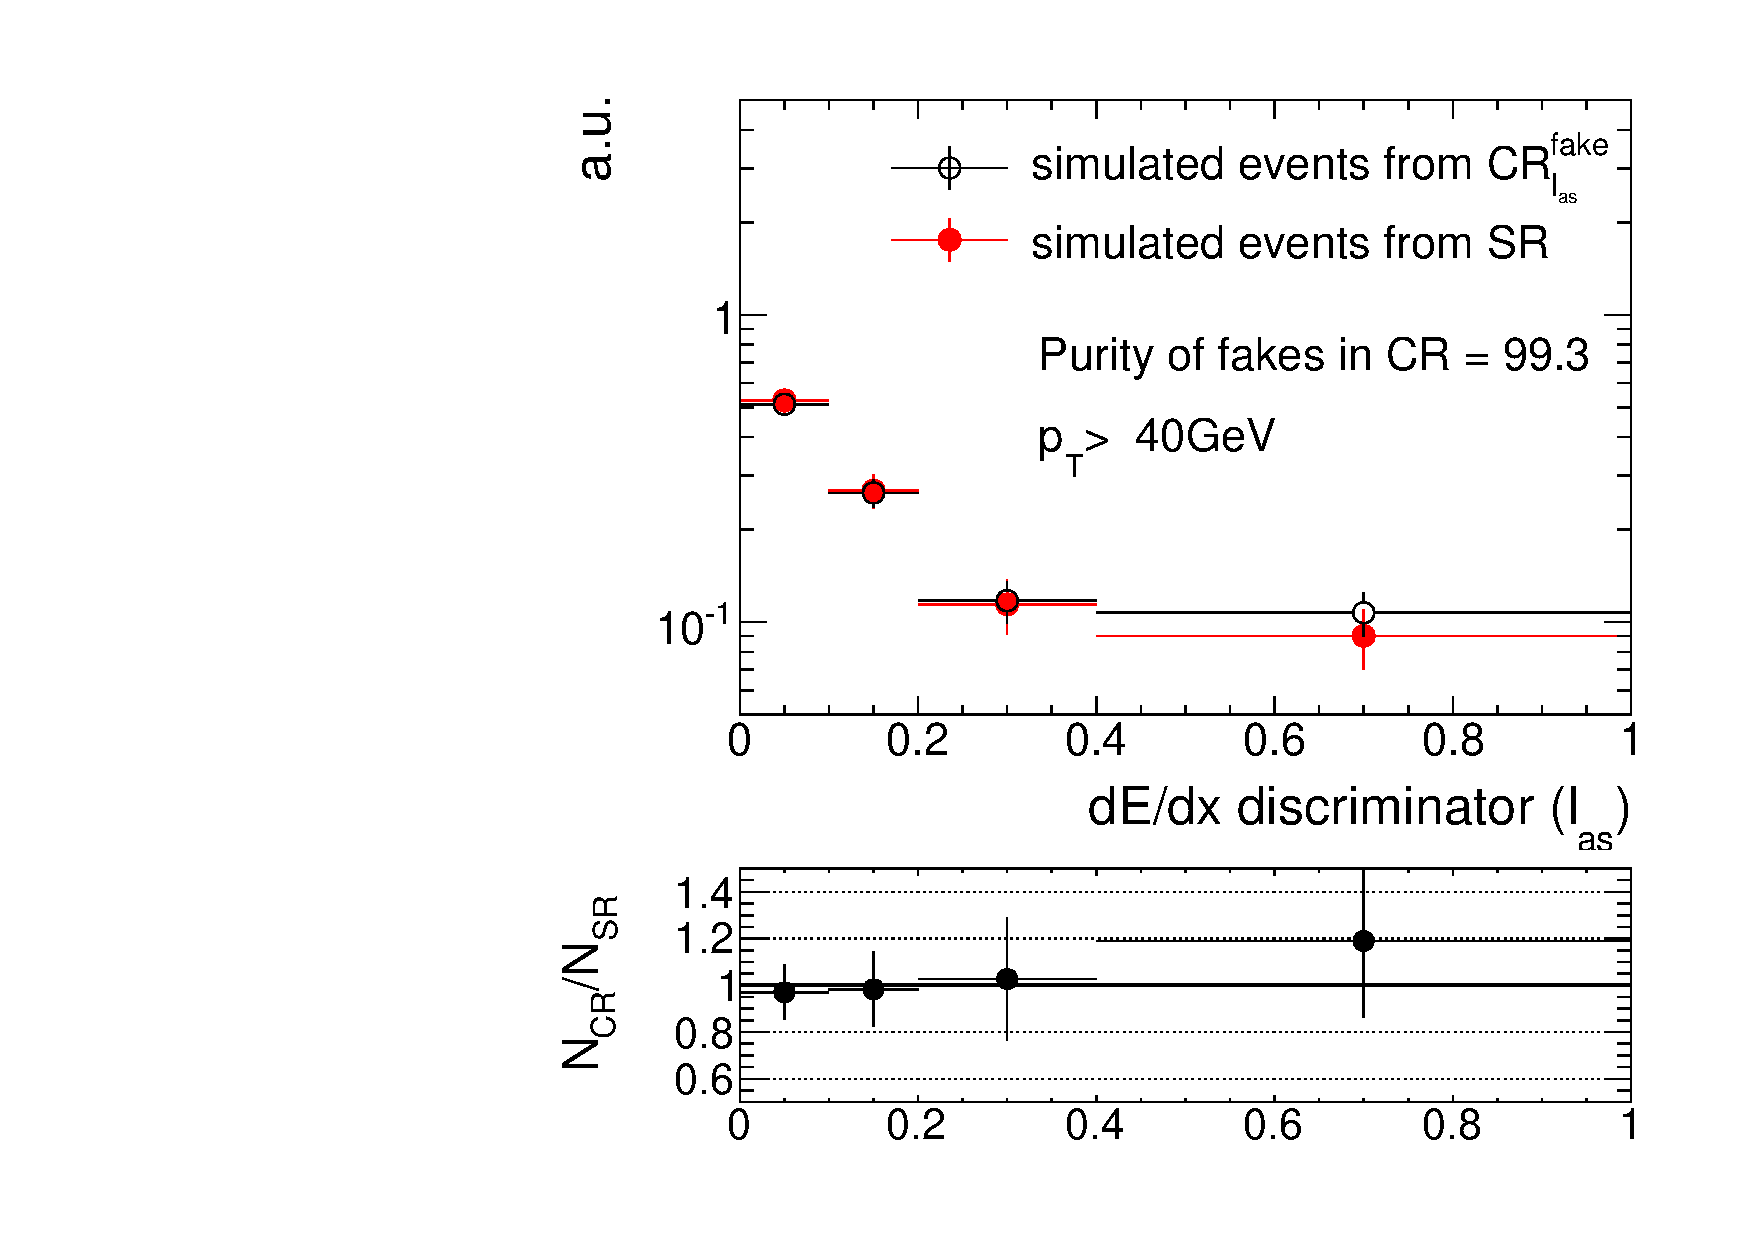
\includegraphics[width=0.49\textwidth]{figures/analysis/Background/hASmi_fakes_ECalaoLe5_trackPtGt40.pdf}
  \end{tabular}
  \caption{Comparison of the \ias shape between \fakeCR and the signal region for two different track \pt selections of $\pt>20\gev$ (left) and $\pt>40\gev$ (right). To enhance the statistical precision only the track-based selection is applied.}
  \label{fig:IasSRCRFakes}
\end{figure}

The \ias shape is almost identical in the signal and in the control region which makes the definition of the control region perfectly for estimating the \ias shape from \fakeCR in data.
The remaining shape differences are taken into account as a systematic uncertainty (discussed in Section~\ref{sec:FakeIasUncertainty}).
%%%%%%%%%%%%%%%%%%%%%%%%%%%%%%%%%%%%%%%%%%%%%%%%%%%%%%%%%%%%%%%%%%%%%%%%%%%%%%%%%%%%%%%%%%%%%%%%%%%%%%%%%%%%%%%%%%%%%%%%%%%%%%%%%%%%%%%%%%%%%%%%%%%%%%%%%%%%%%%%%%%%%%%
%%%%%%%%%%%%%%%%%%%%%%%%%%%%%%%%%%%%%%%%%%%%%%%%%%%%%%%%%%%%%%%%%%%%%%%%%%%%%%%%%%%%%%%%%%%%%%%%%%%%%%%%%%%%%%%%%%%%%%%%%%%%%%%%%%%%%%%%%%%%%%%%%%%%%%%%%%%%%%%%%%%%%%%
%%%%%%%%%%%%%%%%%%%%%%%%%%%%%%%%%%%%%%%%%%%%%%%%%%%%%%%%%%%%%%%%%%%%%%%%%%%%%%%%%%%%%%%%%%%%%%%%%%%%%%%%%%%%%%%%%%%%%%%%%%%%%%%%%%%%%%%%%%%%%%%%%%%%%%%%%%%%%%%%%%%%%%%

\section{Leptonic background}
\label{sec:LeptonicBkg}

The leptonic background of the here presented search is caused by non-reconstructed leptons that circumvent the lepton veto selection.
However, at least non-reconstructed electrons or taus should in principle deposit enough energy in the calorimeters such that they can still be vetoed by the calorimeter isolation requirement $\ecalo<5\gev$.
As muons don't deposit much energy in the calorimeters, this reasoning does not apply to them.
In the following, the sources of the three different leptonic backgrounds are characterised.

\subsection*{Electrons}
To reject unreconstructed electrons, all tracks pointing to a dead or noisy ECAL cell, to an ECAL intermodule gap, or to the region between ECAL barrel and endcap at $1.42<|\eta|<1.65$ are vetoed, 
as described in Section~\ref{sec:AnalysisSelection}.
By this selection, almost all electrons are efficiently rejected.
In the simulated \WJets sample only one simulated event remains that passes all signal candidate selection criteria and for which the candidate track can be matched to a generator-level electron.
This event is visualised in Fig.~\ref{fig:LostElectron}. 
\begin{figure}[!t]
  \centering 
  \begin{tabular}{c}
    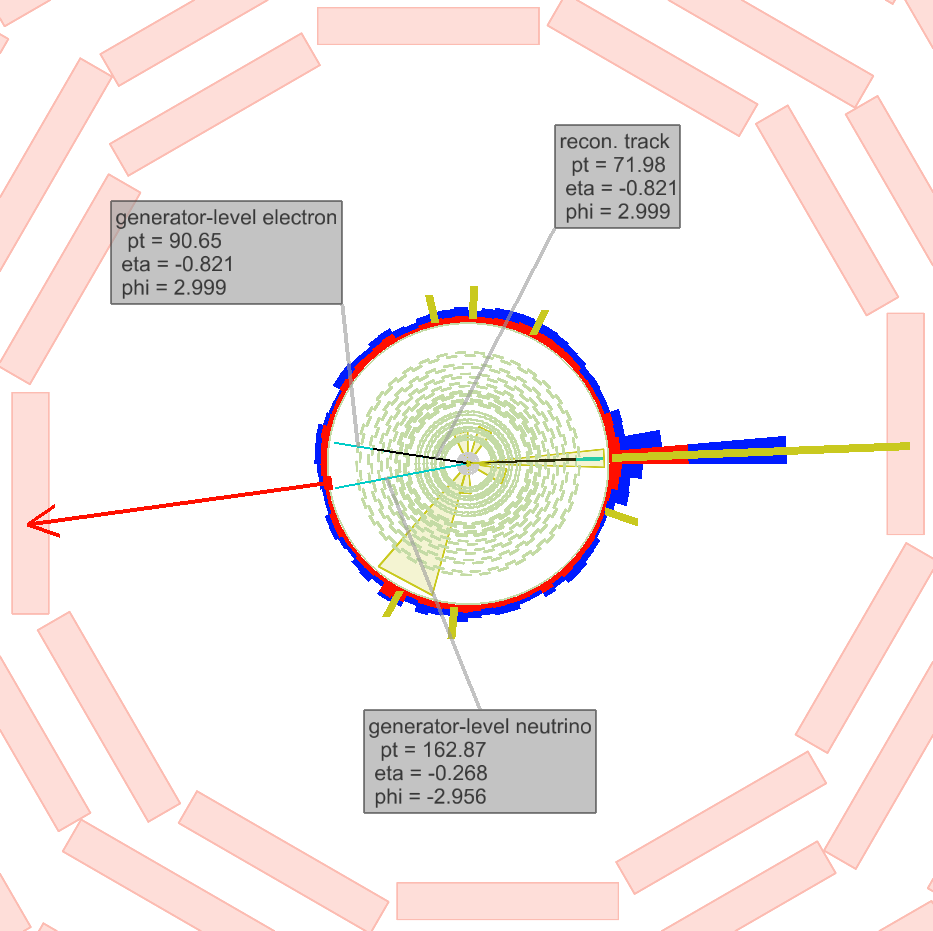
\includegraphics[width=0.49\textwidth]{figures/analysis/Electron_lumi_279317_event_111637553.png}
  \end{tabular}
 \caption{Visualisation of a $W\rightarrow e\nu_e$ event contributing to the SM background. 
           In light blue, generator-level particles including \lel and \nue of the \W-boson decay are shown. 
           The neutrino, only weakly interacting does not show any signature in the detector, whereas the electron ($\pt\simeq 90\gev$) leaves a track (black line) with \mbox{$\pt\simeq 70\gev$} in the tracker. 
           No ECAL energy deposits in the direction of the electron are visible. 
           This is caused by the fact that the corresponding ECAL energy deposits were not read out in this event.
           An ISR jet ($\pt\simeq 230\gev$) causes the \met (read arrow) in the event. }
  \label{fig:LostElectron}
\end{figure}
 
In this event no energy deposits in the ECAL are read out, which suggests that the corresponding ECAL tower was not working properly in 2012.
Additionally, electrons can do bremsstrahlung which can change the direction of the electron significantly.
Thus, the energy deposits in the ECAL can possibly not be matched to the original electron.

\subsection*{Taus}
Taus are contributing to the leptonic background through the hadronic decay of a tau lepton to one charged pion $\tau\rightarrow\pi^{\pm}\nu_{\tau}$.
Other decay modes of the tau lepton are suppressed by the track isolation criterion.
Taus fail reconstruction if they don't deposit energy in the HCAL or ECAL.
Unreconstructed taus can therefore also easily bypass the calorimeter isolation criterion.
Because of nuclear interactions in the tracker, pions often result in short reconstructed tracks that can easily be highly mismeasured in \pt.
Thus, taus can contribute to the background even if imposing a tight selection in the transverse momentum.
Such an event is shown in Fig.~\ref{fig:LostTau}.  
\begin{figure}[!tb]
  \centering 
  \begin{tabular}{c}
    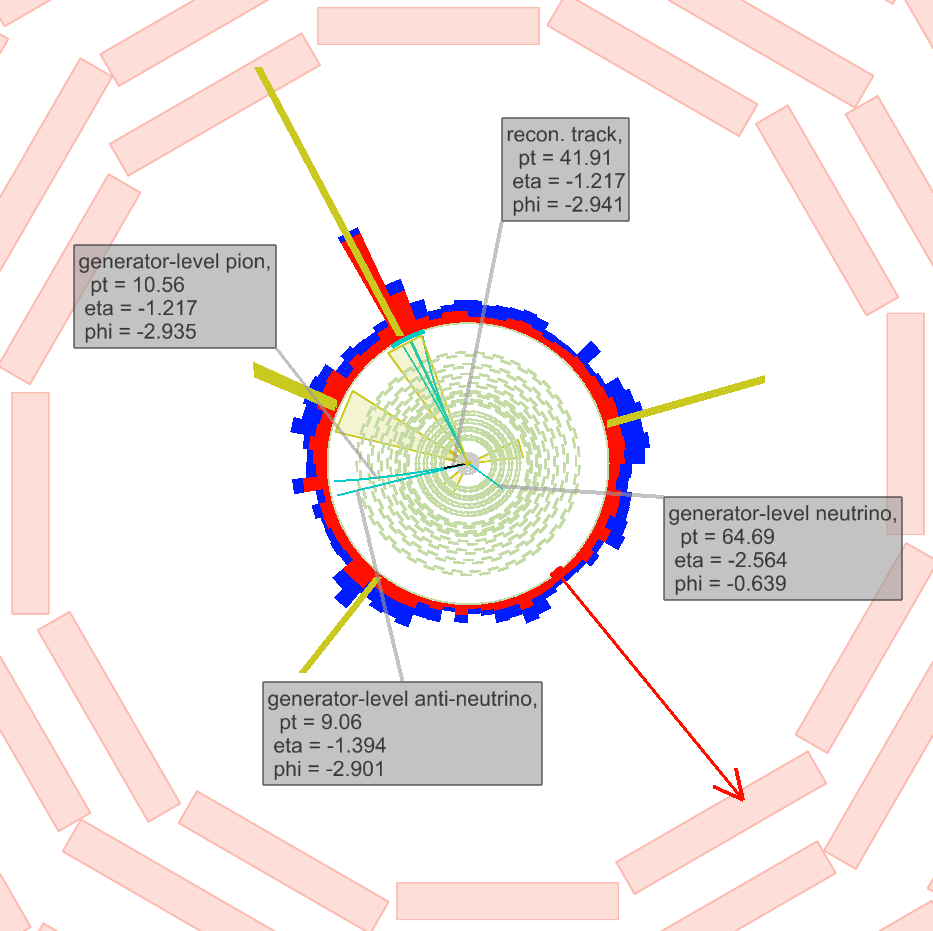
\includegraphics[width=0.49\textwidth]{figures/analysis/Background/LostTau_lumi_20940_event_8369426.png}
  \end{tabular}
  \caption{Visualisation of a $W^{+}\rightarrow \tau^{+}\nu_{\tau} \rightarrow \pi^{+}\bar{\nu}_{\tau} \nu_{\tau} $ event contributing to the SM background. 
           In light blue, the generator-level particles including $\pi^{+}$, $\bar{\nu}_{\tau}$ and $\nu_{\tau}$ are shown.
           The transverse momentum of the generator-level pion is only $\pt\sim10\gev$, but because the reconstructed track (black line) is very short, it leads to a high mismeasurement of the track \pt of $\sim40\gev$.
           The shortness of the track is caused by nuclear interactions of the pion.
           As no corresponding ECAL or HCAL energy deposits are measured, the reconstruction of the pion fails.
           The ISR jet causes the \met (read arrow) in the event. }
  \label{fig:LostTau}
\end{figure}

\subsection*{Muons}
Muons can fail reconstruction if they point towards a bad cathode strip chamber.
This is taken into account in the candidate track selection.
However, some of the muons still fail reconstruction if they fall within the gap between stations 0 and 1 of the drift tube system at $|\eta|=0.25$.
The muon reconstruction efficiency drops from around 99\% to a value of around 94\% as shown in~\cite{bib:CMS:DT_Thesis,bib:CMS:DT_8TeV_AN}.
This possibility is illustrated in a simulated event shown in Fig.~\ref{fig:LostMuon}.
\begin{figure}[!tb]
  \centering 
  \begin{tabular}{c}
    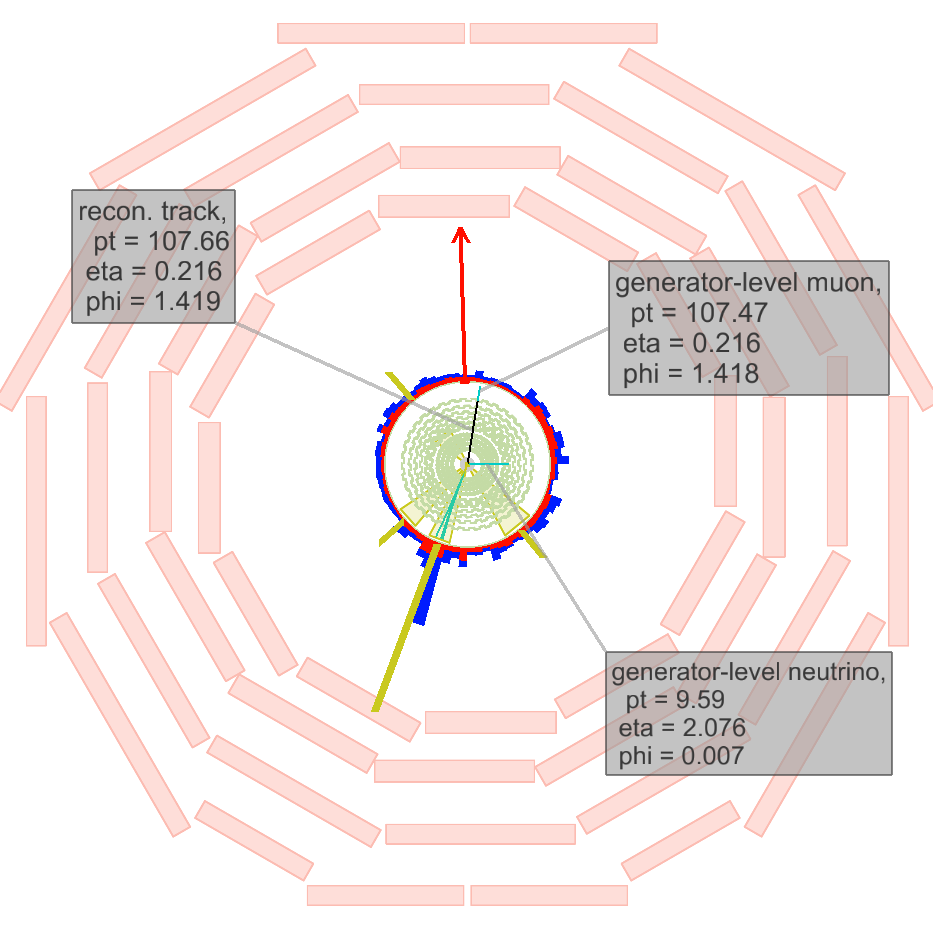
\includegraphics[width=0.49\textwidth]{figures/analysis/Background/LostMuon_Lumi_456307_event_182377157_NEW.png}
  \end{tabular}
  \caption{Visualisation of an $W\rightarrow \mu\nu_{\mu}$ event contributing to the SM background. 
           In light blue, the generator-level particles including $\mu$ and $\nu_{\mu}$ of the $W$ decay are shown. 
           The muon is pointing to the $\eta$-region between stations 0 and 1 of the DT system at $|\eta|\sim0.25$.
           In this region the muon reconstruction is less efficient. No signal in the muon chambers is visible. Therefore the muon could not be reconstructed.
           The ISR jet causes the \met (read arrow) in the event.}
  \label{fig:LostMuon}
\end{figure}


In~\cite{bib:CMS:DT_Thesis,bib:CMS:DT_8TeV_AN} events are rejected if the track is pointing in a region of $0.15<|\eta|<0.35$.
In this search, this cut was omitted to maximise signal acceptance. 
Due to the additional selection in \ias, muons can be efficiently suppressed.
E.g. in the event shown in Fig.~\ref{fig:LostMuon}, the muon has an \ias value of about 0.007.\\

In general, all leptons are minimally ionising.
However, as electrons are much lighter compared to muons or pions, they loose more energy also via radiative effects.
Still, all three lepton types loose much less energy compared to hypothetical new heavy particles.
To have the possibility to make an optimisation in the two main discriminating variables \pt and \ias, the background estimation methods are designed to work for all different \pt and \ias selection cuts.\\

%A comparison of the \ias distribution for all four different background sources is shown in Fig.~\ref{fig:IasDist}.




As for the fakes, the leptonic background estimation is splitted into two parts.
First, the estimation of the inclusive background without \ias information.
Second, the estimation of the \ias shape for all three leptonic background sources.


\subsection{Inclusive leptonic background estimation}
The inclusive (without \ias information) lepton background estimation method is similar to the background estimation method used in~\cite{bib:CMS:DT_Thesis,bib:CMS:DT_8TeV_AN}.

In order to estimate the number of events in the signal region originating from unreconstructed leptons, information from simulated events is used.
With the help of simulated \WJets events, the ratio \leptonscalefactor between the number of events in the signal region with the selected track matched to a generator-level lepton $N_{SR}^{\text{trk matched to lepton}_i}$
 and the number of events in a control region $N_{CR}^{\text{lepton}_i\text{ veto inverted}}$ with a inverted lepton veto is determined.
For muons, this lead to the following expression
\begin{equation*}
\rho_{\text{MC}}^{\mu} = \frac{N_{\text{SR,MC}}^{\text{trk matched to }\mu}}{N_{\text{CR,MC}}^{\mu \text{ veto inverted}}}.
\end{equation*}
Since for electrons and taus the reconstruction efficiency is highly correlated with the \ecalo selection requirement, the \ecalo requirement is additionally removed in the control regions for these two lepton types 
\begin{equation*}
\rho_{\text{MC}}^{e,\tau} = \frac{N_{\text{SR,MC}}^{\text{trk matched to }e,\tau}}{N_{\text{CR,MC}}^{e,\tau\text{ veto inverted}, \cancel{\ecalo<5\gev}}}.
\end{equation*}

In order to estimate the inclusive background for all three lepton types, the scaling factor \leptonscalefactor is applied to the number of events in the lepton veto inverted control region measured in data.
Also in data the control region for electrons and taus is defined with the \ecalo requirement removed. 
Thus, the inclusive number of predicted background events can be estimated with  
\begin{equation*}
N^{\mu \text{, inclusive in I$_{\text{as}}$}}_{\text{bkg}} = \rho_{\text{MC}}^{\mu} \cdot N_{\text{CR,data}}^{\mu\text{ veto inverted}}.
\end{equation*}
for muons, and 
\begin{equation*}
N^{e,\tau\text{, inclusive in I$_{\text{as}}$}}_{\text{bkg}} = \rho_{\text{MC}}^{e,\tau} \cdot N_{\text{CR,data}}^{e,\tau\text{ veto inverted}, \cancel{\ecalo<5\gev}}.
\end{equation*}
for electrons and taus.

This method relies on the simulation of the lepton reconstruction efficiencies which is expected to be reasonably accurate~\cite{bib:CMS:elec_recoEff,bib:CMS:muon_recoEff,bib:CMS:tau_recoEff}.
For electrons and taus the simulation of the calorimeter isolation is utilised as well.
Possible discrepancies between simulation and data are taken into account as a systematic uncertainty via a comparison of the lepton reconstruction efficiencies in data and simulation in \Zlep events (see Section~\ref{sec:LeptonScaleUncertainty}).

To reduce the statistical uncertainty, the scale factor is calculated without applying the QCD suppression cuts. 
After the signal candidate selection described in Section~\ref{sec:AnalysisSelection}, only one event remains in the simulated \WJets sample where the candidate track can be matched to an electron.
There are five track candidates that can be matched to a muon, and zero selected tracks that can be matched to a pion.
The statistical uncertainties are calculated as the 68\% upper and lower limits on the inclusive background with the Neyman procedure~\cite{bib:Neyman_1937,bib:PDG_2014}.
Table~\ref{tab:LeptonicResults} gives the result for the prediction of the inclusive leptonic background for the signal candidate selection from Section~\ref{sec:AnalysisSelection}.

\renewcommand{\arraystretch}{1.5}
\begin{table}[!h]
\centering
\caption{Scaling factor \leptonscalefactor, number of events in the data control region N$_{\text{CR,data}}$ and the resulting inclusive estimation N$_{\text{predicted}}$ after the candidate track selection.}
\label{tab:LeptonicResults}
\makebox[0.99\textwidth]{
\begin{tabular}{l|c |c| c }
\multicolumn{4}{c}{} \\
\toprule
                                                               &      scaling factor \leptonscalefactor    &   N$_{\text{CR,data}}$         &  N$_{\text{predicted}}$   \\
\midrule
electrons                                                      &       $1.25^{+1.70}_{-0.77} \cdot 10^{-4}  $      & 60067                     & $7.49^{+10.19}_{-4.63}$     \\
muons                                                          &       $2.17^{+1.65}_{-0.93} \cdot 10^{-4}$        & 76664                     & $16.64^{+12.64}_{-7.12}$    \\
taus                                                           &       $< 2.13 \cdot 10^{-2}$                  & 445                      &  $<9.46$ \\
\bottomrule
\multicolumn{4}{c}{} \\
\end{tabular}}
\end{table}



\subsection{dE/dx shape of leptonic background}
In order to get information about the \ias (see Section~\ref{sec:Ias}) shape in the signal region of electrons, muons and taus, a control region must be found where the shape of the observable is at least similar to that in the
signal region.
The most natural control region, being the lepton veto inverted control region, cannot be used because the variable \ias is highly correlated to the lepton reconstruction efficiency, as can be seen in Fig.~\ref{fig:LeptonIasDist}.
\begin{figure}[!tb]
  \centering 
  \begin{tabular}{c}
    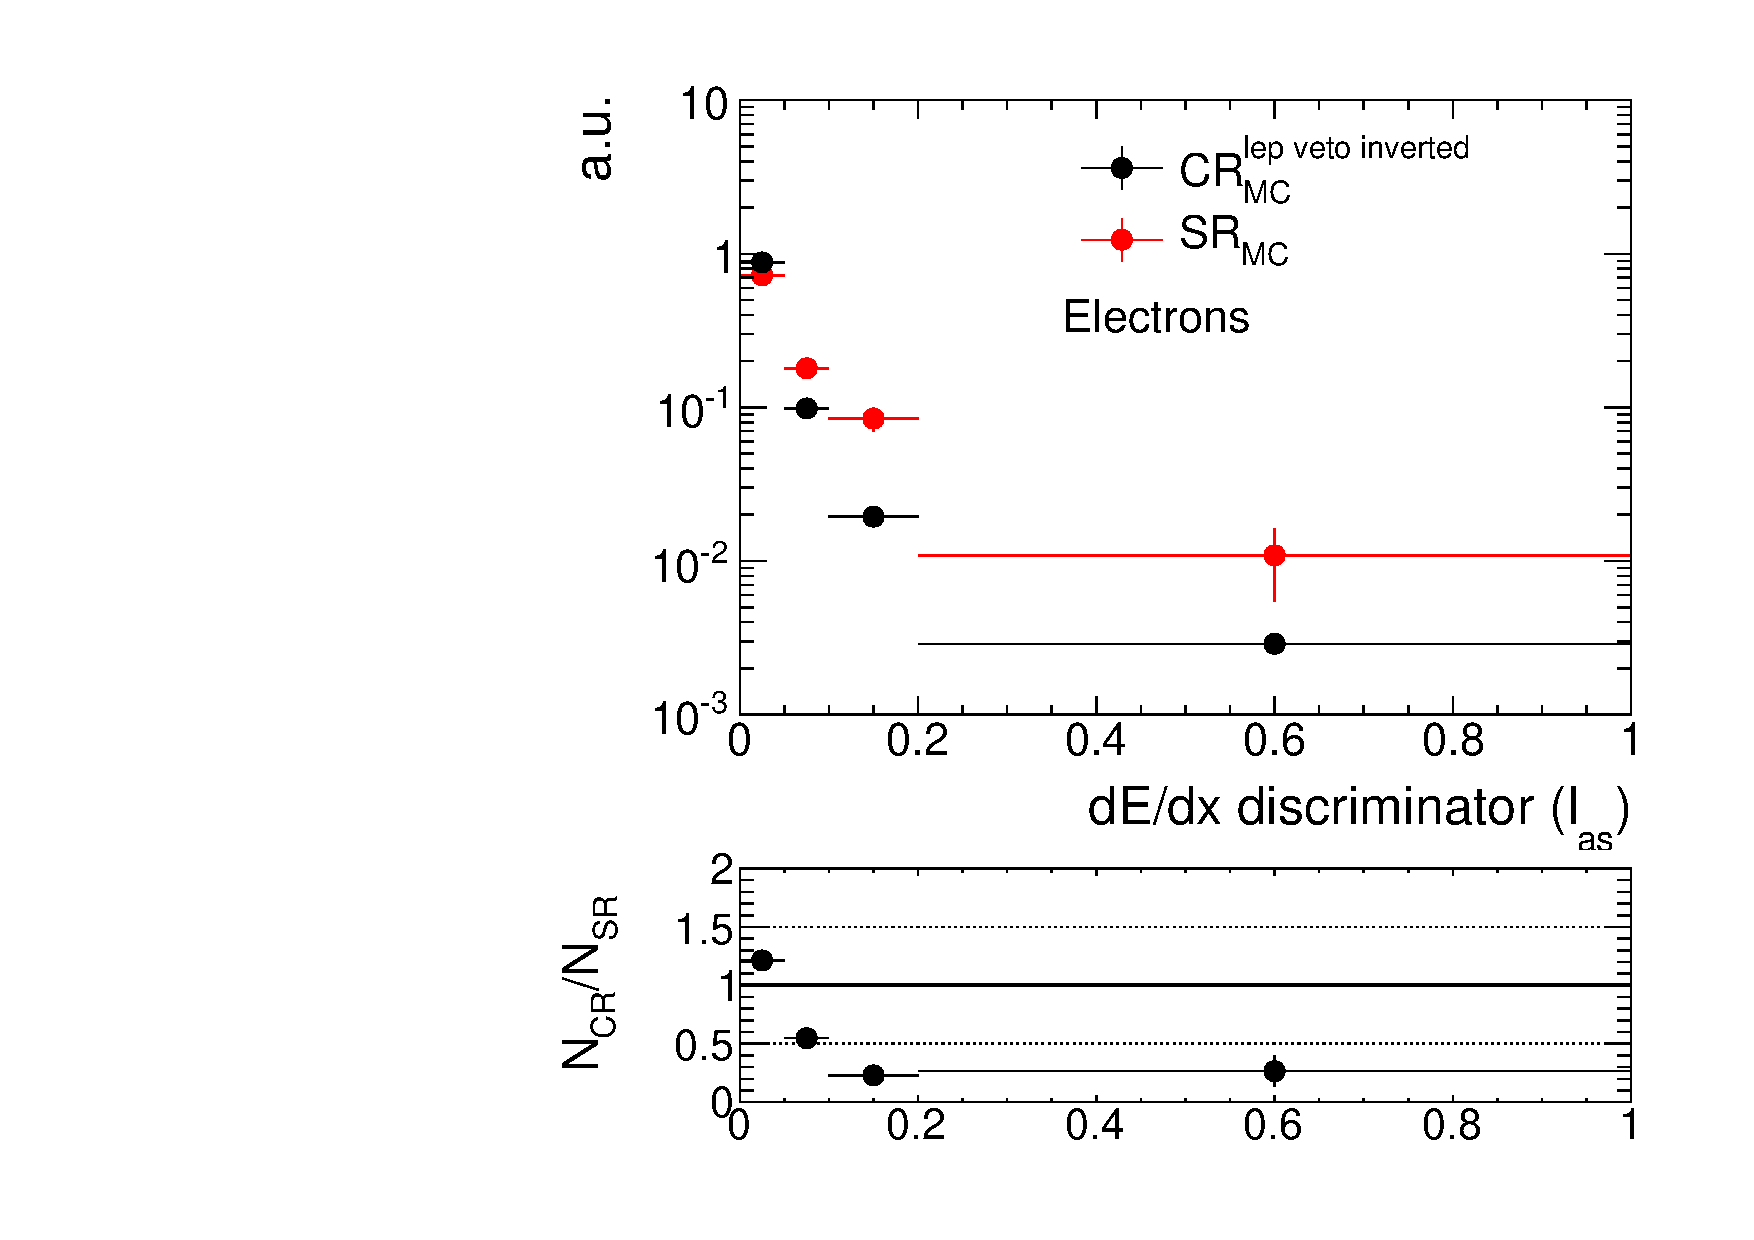
\includegraphics[width=0.33\textwidth]{figures/analysis/Background/hASmi_Electrons_MCCR_MCSR.pdf}
    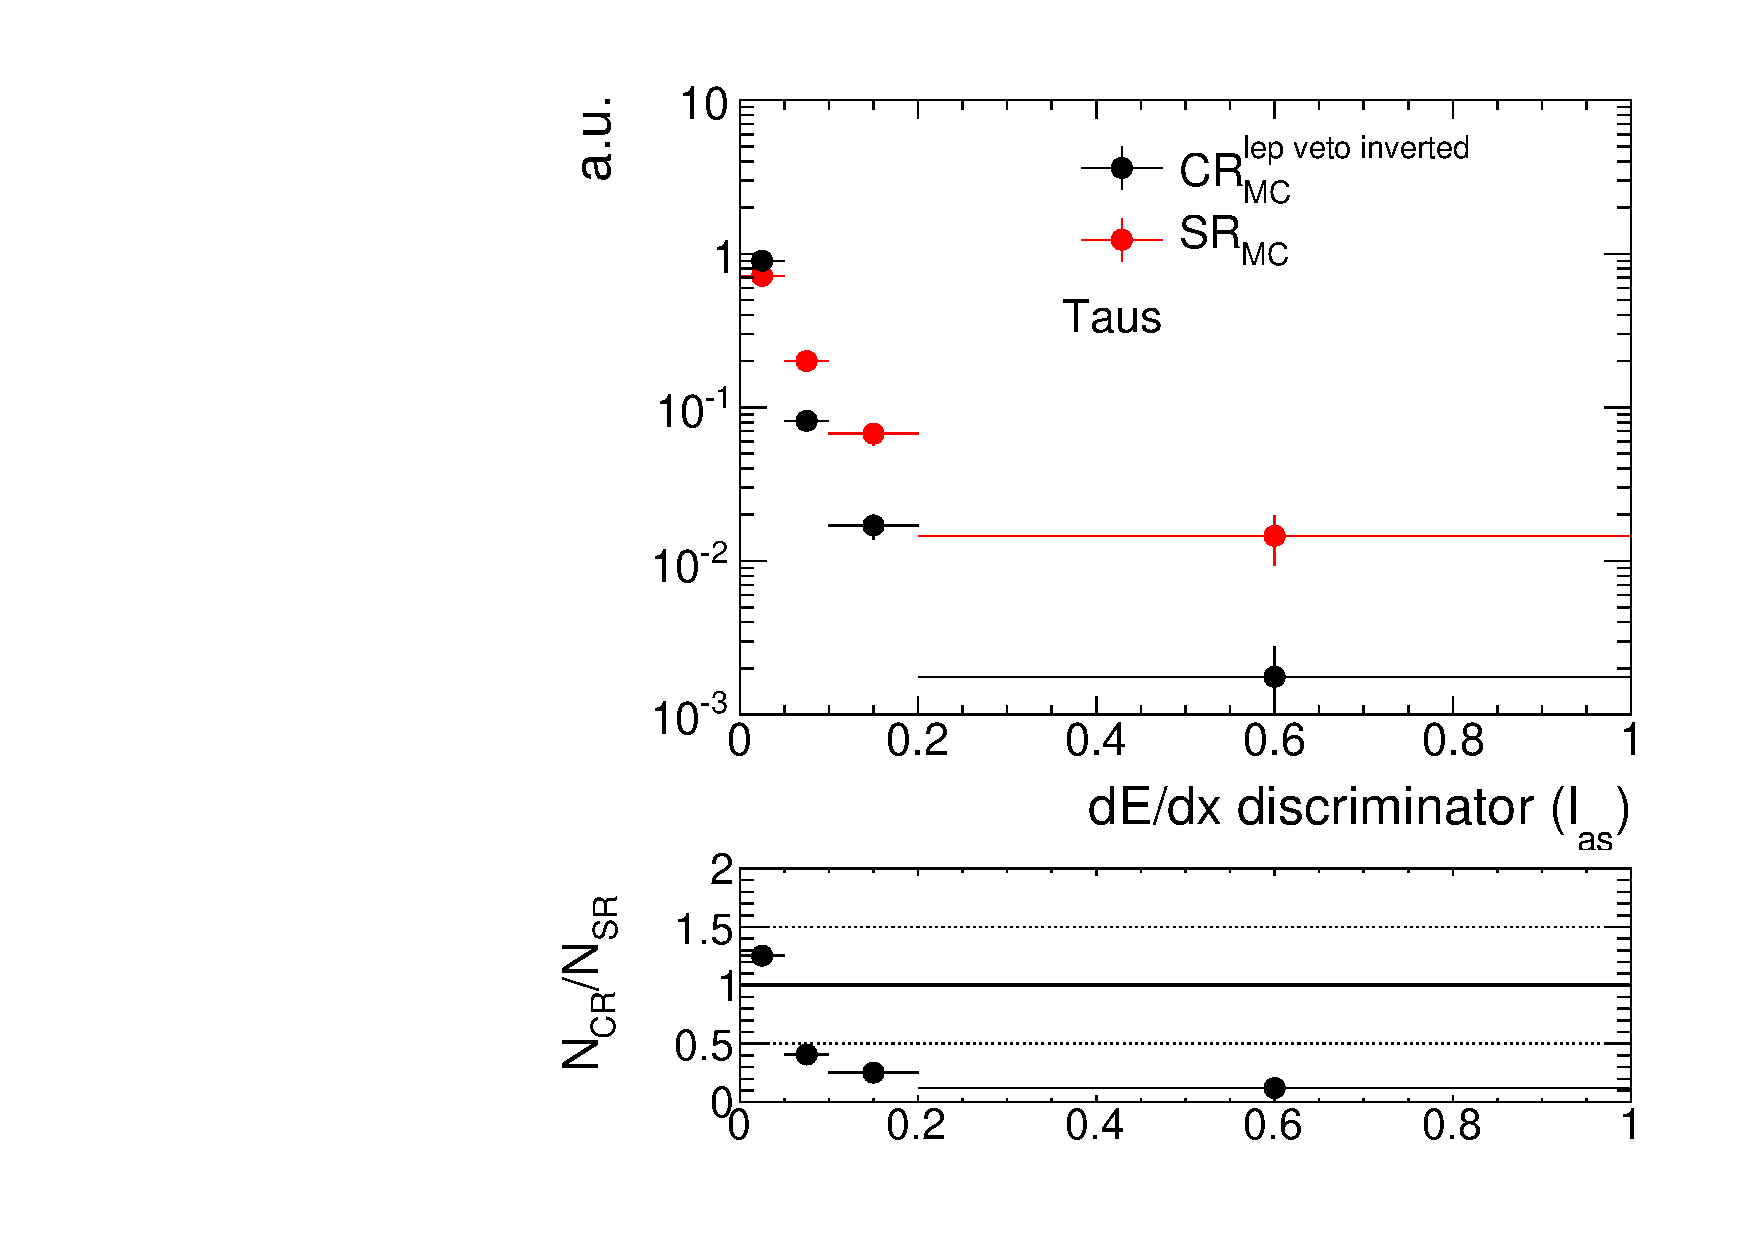
\includegraphics[width=0.33\textwidth]{figures/analysis/Background/hASmi_Taus_MCCR_MCSR.pdf}
    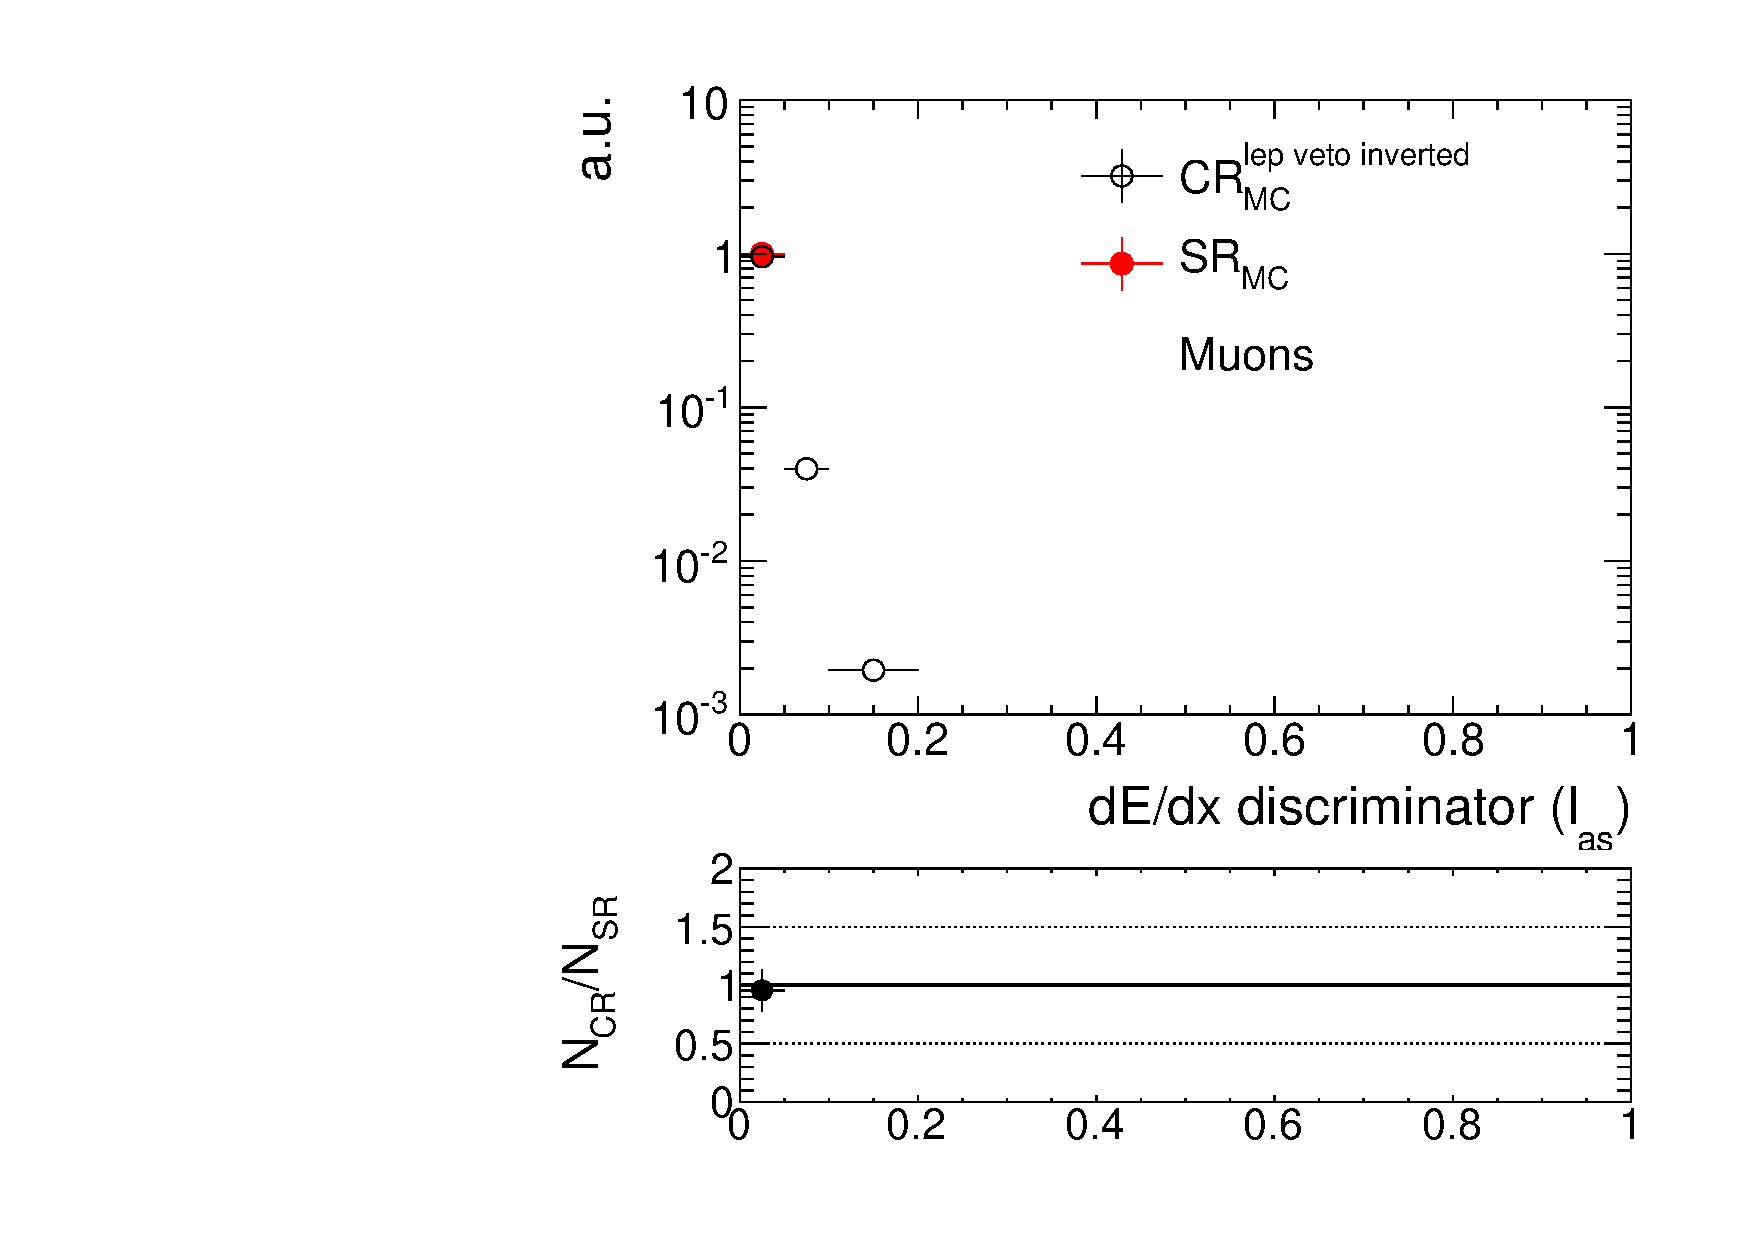
\includegraphics[width=0.33\textwidth]{figures/analysis/Background/hASmi_Muons_MCCR_MCSR.pdf}
  \end{tabular}
  \caption{Normalised \ias distribution for electrons (left), pions from the tau decay (middle) and muons (right) in the signal region (red) and the lepton veto inverted control region (black).}
  \label{fig:LeptonIasDist}
\end{figure}
The discrepancies reach factors up to an order of magnitude.

Various other control regions were tested and could not be used because of too large \ias shape differences to the signal region.

As no suitable control region exists where the \ias shape of the leptons is at least similar to the shape in the signal region, it is decided to use the \ias information from simulation.
This introduces a large systematic uncertainty since \dedx (and therefore \ias) is not simulated well.
However, the corresponding systematic uncertainty is still smaller than taking the \ias shape from a control region in data: compare Fig.~\ref{fig:LeptonIasDist} and Fig.~\ref{fig:LeptonIasDistData}.
\begin{figure}[!tb]
  \centering 
  \begin{tabular}{c}
    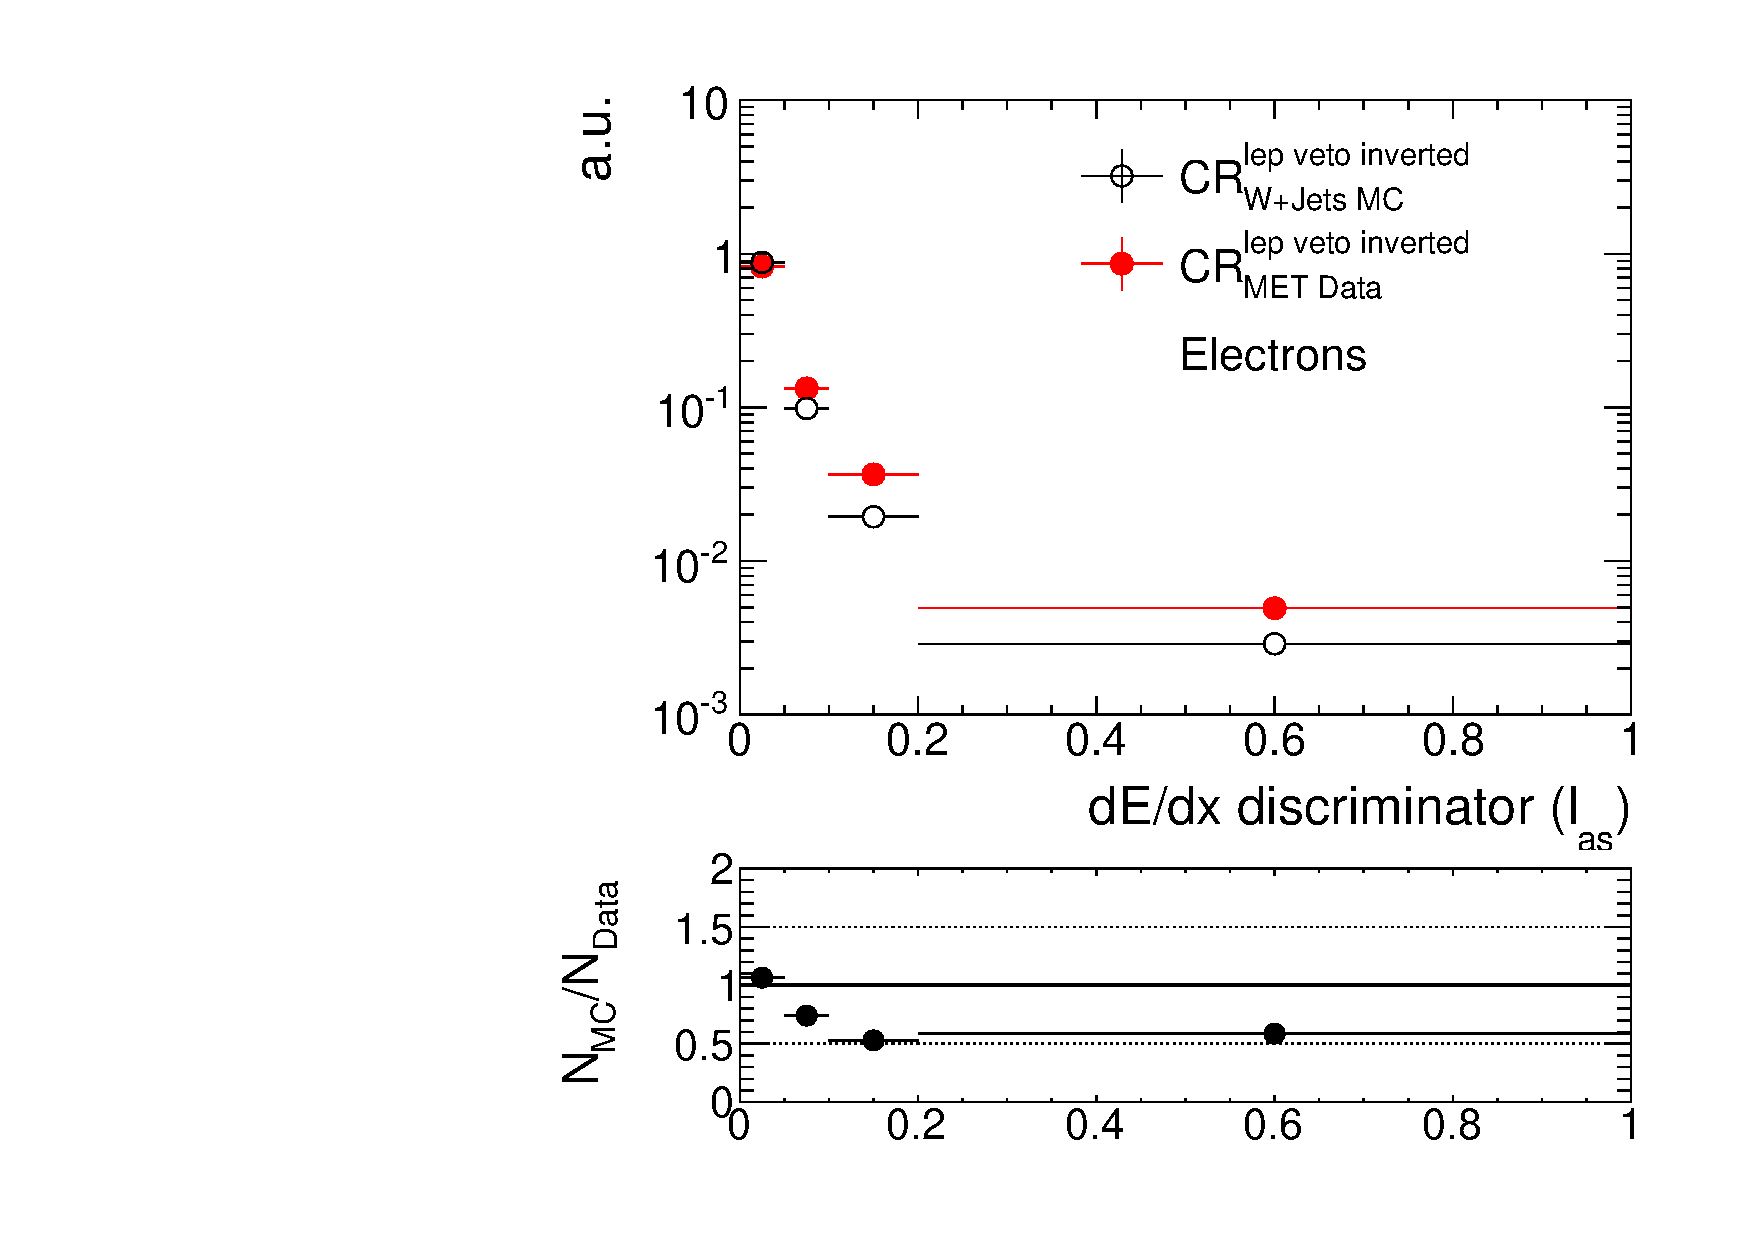
\includegraphics[width=0.33\textwidth]{figures/analysis/Background/hASmi_Electrons_MCCR_DataCR.pdf}
    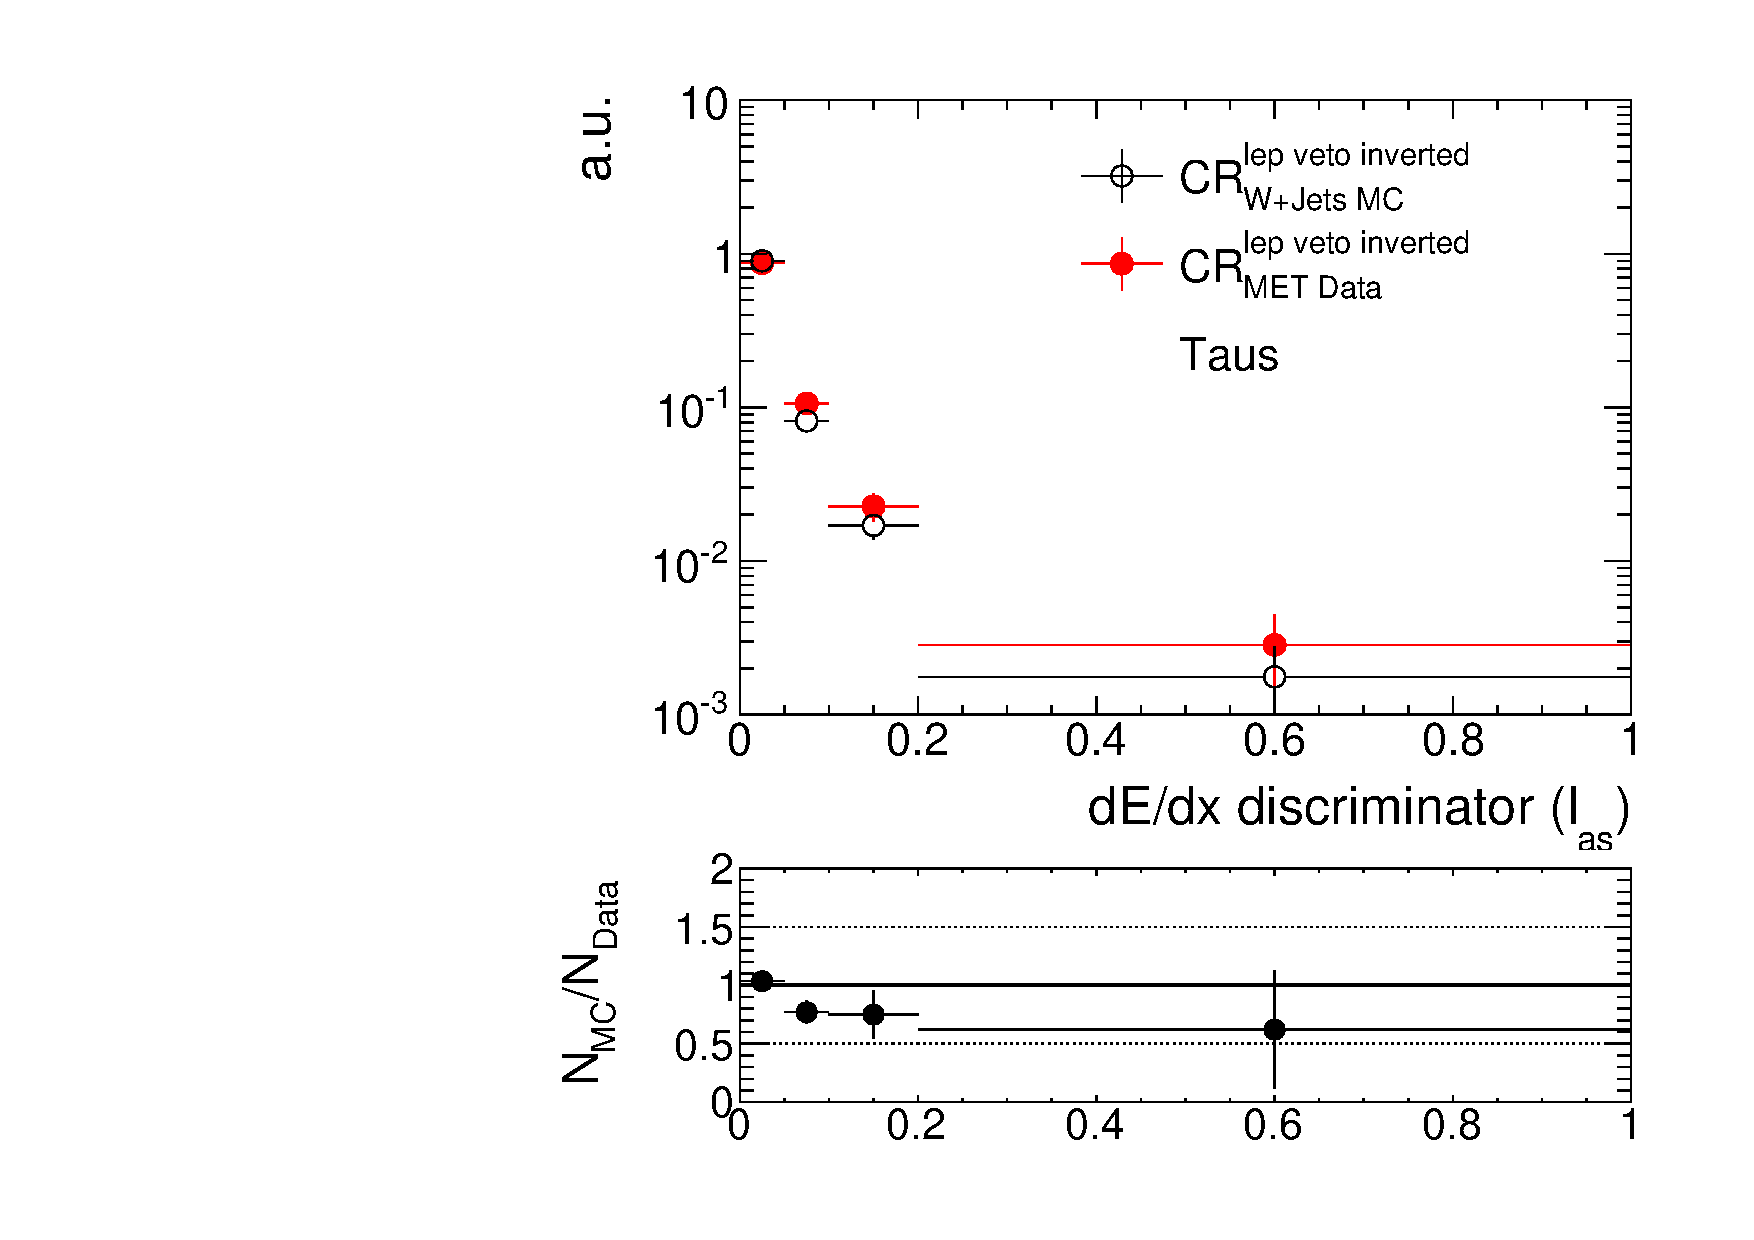
\includegraphics[width=0.33\textwidth]{figures/analysis/Background/hASmi_Taus_MCCR_DataCR.pdf}
    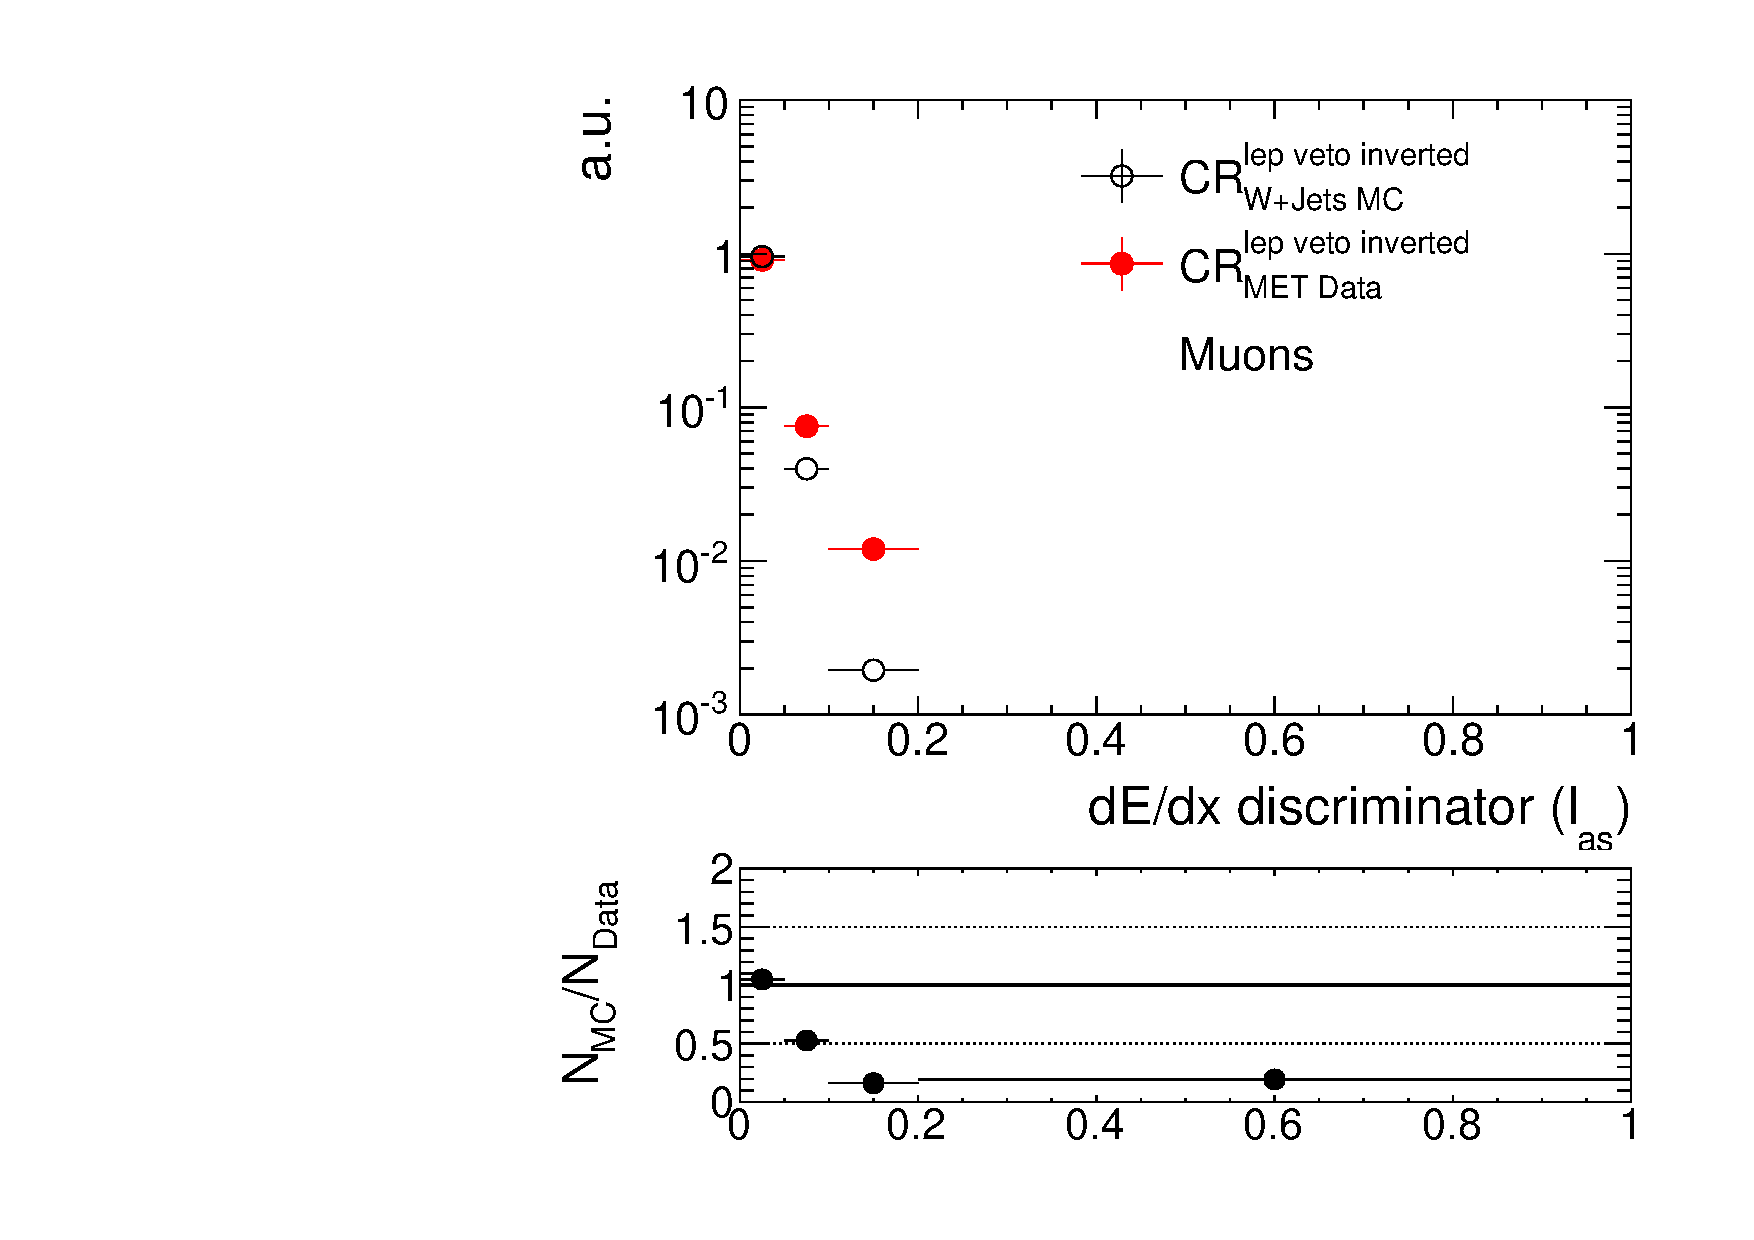
\includegraphics[width=0.33\textwidth]{figures/analysis/Background/hASmi_Muons_MCCR_DataCR.pdf}
  \end{tabular}
  \caption{Normalised \ias distribution for electrons (left), pions from the tau decay (middle) and muons (right) in the lepton veto inverted control region from simulated (black) and real (red) events.}
  \label{fig:LeptonIasDistData}
\end{figure}

In order to take into account the bias when using \ias from simulation, a systematic uncertainty is estimated that addresses simulation-data differences of the \ias distributions.
This systematic uncertainty is discussed in Section~\ref{sec:LeptonIasUncertainty}.
%%%%%%%%%%%%%%%%%%%%%%%%%%%%%%%%%%%%%%%%%%%%%%%%%%%%%%%%%%%%%%%%%%%%%%%%%%%%%%%%%%%%%%%%%%%%%%%%%%%%%%%%%%%%%%%%%%%%%%%%%%%%%%%%%%%%%%%%%%%%%%%%%%%%%%%%%%%%%%%%%%%%%%%
%%%%%%%%%%%%%%%%%%%%%%%%%%%%%%%%%%%%%%%%%%%%%%%%%%%%%%%%%%%%%%%%%%%%%%%%%%%%%%%%%%%%%%%%%%%%%%%%%%%%%%%%%%%%%%%%%%%%%%%%%%%%%%%%%%%%%%%%%%%%%%%%%%%%%%%%%%%%%%%%%%%%%%%
\section{Background estimation validation}
\label{sec:BkgValidation}

The background estimation methods are exhaustively validated with the help of signal depleted control regions.
Various control regions are used for validation.

First, to validate the estimation method of the leptonic background, a leptonic control region is defined by selecting only tracks with a minimum number of seven hits in the tracker.
This reduces the fake contribution to a minimum (cf. Fig.~\ref{fig:NValidFakes}).
Additionally in order to minimise signal contamination, the calorimeter isolation requirement is inverted to $\ecalo>10\gev$.
The validation test for the control region with $\ecalo>10\gev$ and $\nhits>6$ is shown in Table~\ref{tab:LeptonicClosure}.
The predicted number of events by the leptonic background estimation is compatible with the observed data yield.\\
\renewcommand{\arraystretch}{1.5}
\begin{table}[!h]
\centering
\caption{Validation test of leptonic background estimation. Left: $\ecalo>10\gev$ and $\nhits>6$. Right: $\ecalo>10\gev$, $\nhits>6$ and $\ias>0.2$. Only statistical uncertainties are included.}
\label{tab:LeptonicClosure}
\makebox[0.99\textwidth]{
\begin{tabular}{l|c |c}
\multicolumn{3}{c}{} \\
\toprule
                                                               &      Predicted Yield                       &   Data Yield          \\
\midrule
Total bkg                                                      &       $132.68^{ + 26.31}_{-18.43}$         &  156        \\
\midrule
Electrons                                                      &       $14.67^{+ 11.16}_{-6.29}$            &                \\
Muons                                                          &       $7.99^{ + 10.90}_{-5.00}$            &            \\
Taus                                                           &       $109.04^{+21.18}_{-16.58}$           &          \\


\bottomrule
\multicolumn{3}{c}{} \\
\end{tabular}
\hspace{10pt}
\begin{tabular}{l|c |c}
\multicolumn{3}{c}{} \\
\toprule
                                                               &      Predicted Yield                   &   Data Yield          \\
\midrule
Total bkg                                                      &       $0.0^{+ 0.50}_{-0.0}$               &  1        \\
\midrule
Electrons                                                      &       $0.0^{+ 0.07}_{-0.0}$               &                \\
Muons                                                          &       $0.0^{+ 0.32}_{-0.0}$               &            \\
Taus                                                           &       $0.0^{+ 0.38}_{-0.0}$               &          \\


\bottomrule
\multicolumn{3}{c}{} \\
\end{tabular}}
\end{table}


As the fake background can only be estimated within the low calorimeter isolation region $\left(\ecalo<10\gev\right)$ to ensure high fake purity, 
the information about the number of fake tracks in the high calorimeter isolation region is taken from the fake enriched control region \fakeCR defined in Section~\ref{sec:FakeBkg}.
In this control region, the ratio of $N_{\ecalo>10\gev}/N_{\ecalo<10\gev}$ is estimated and taken as a multiplicand to the number of events predicted from the $\ecalo<10\gev$ region.
In Table~\ref{tab:FakeClosure}, two different validation tests are shown, once an inclusive validation in \ias and once with an \ias selection of 0.2.
Again, the predicted background events is in agreement with the number of observed events.
\renewcommand{\arraystretch}{1.5}
\begin{table}[!b]
\centering
\caption{Validation test of fake and leptonic background estimation methods. Left: $\ecalo>10\gev$ . Right: $\ecalo>10\gev$ and $\ias>0.2$. Only statistical uncertainties are included.}
\label{tab:FakeClosure}
\makebox[0.99\textwidth]{
\begin{tabular}{l|c |c}
\multicolumn{3}{c}{} \\
\toprule
                                                               &      Predicted Yield                   &   Data Yield          \\
\midrule
Total bkg                                                      &     $309.00^{+ 33.46} _{- 26.62}$             &  324        \\
\midrule
Electrons                                                      &     $59.92^{ + 16.11}_{ - 11.85}$                 &                \\
Muons                                                          &     $8.04^{ + 10.97}_{ - 5.03}$                &            \\
Taus                                                           &     $173.06^{+ 24.62}_{- 20.23}$               &          \\
Fakes                                                          &     $67.98^{+ 11.57}_{- 11.57}$               &          \\
\bottomrule
\multicolumn{3}{c}{} \\
\end{tabular}
\hspace{10pt}
\begin{tabular}{l|c |c}
\multicolumn{3}{c}{} \\
\toprule
                                                               &      Predicted Yield                       &   Data Yield          \\
\midrule
Total bkg                                                      &       $14.80^{ + 2.92}_{- 2.85}$            &  16        \\
\midrule
Electrons                                                      &       $0.75^{ + 0.36}_{ - 0.25}$            &                \\
Muons                                                          &       $0.00^{ + 0.32}_{- 0.00}$            &            \\
Taus                                                           &       $2.33^{ + 0.74}_{- 0.55}$            &          \\
Fakes                                                          &       $11.72^{ + 2.79}_{- 2.79}$            &          \\
\bottomrule
\multicolumn{3}{c}{} \\
\end{tabular}}
\end{table}


The whole validation is done for different selections in \pt and \ias.
All validation tests show good agreement and can be found in Appendix~\ref{app:Validation}.

Still, systematic uncertainties need to be estimated.
The sources of systematic uncertainties and how they are estimated will be explained in the following section.

%%%%%%%%%%%%%%%%%%%%%%%%%%%%%%%%%%%%%%%%%%%%%%%%%%%%%%%%%%%%%%%%%%%%%%%%%%%%%%%%%%%%%%%%%%%%%%%%%%%%%%%%%%%%%%%%%%%%%%%%%%%%%%%%%%%%%%%%%%%%%%%%%%%%%%%%%%%%%%%%%%%%%%%
%%%%%%%%%%%%%%%%%%%%%%%%%%%%%%%%%%%%%%%%%%%%%%%%%%%%%%%%%%%%%%%%%%%%%%%%%%%%%%%%%%%%%%%%%%%%%%%%%%%%%%%%%%%%%%%%%%%%%%%%%%%%%%%%%%%%%%%%%%%%%%%%%%%%%%%%%%%%%%%%%%%%%%%
\section{Systematic uncertainties}
\label{sec:SysUncertaintiesBkg}

Systematic uncertainties on the background estimation include:
\begin{itemize}
\item the uncertainty on the fake rate \fakerate;
\item the uncertainty on the \ias shape of fake tracks predicted from a control region;
\item the uncertainty on the leptonic scale factor \leptonscalefactor determined with simulated events;
\item the uncertainty on the \ias shape of the leptonic background.
\end{itemize}

%%%%%%%%%%%%%%%%%%%%%%%%%%%%%%%%%%%%%%%%%%%%%%%%%%%%%%%%%%%%%%%%%%%%%%%%%%%%%%%%%%%%%%%%%%%%%%%%%%%%%%%%%%%%%%%%%%%%%%%%%%%%%%%%%%%%%%%%%%%%%%%%%%%%%%%%%%%%%%%%%%%%%%%
\subsection{Uncertainty on the fake rate}
\label{sec:FakeRateUncertainty}
The fake rate \fakerate is determined with the help of observed \Zlep events.
To estimate the uncertainty on this fake rate caused by differences in the fake rate between different underlying processes, a comparison between the fake rate in simulated \ZlepJets and simulated \WJets events is done.
The fake rate in the $Z\rightarrow\ell \bar{\ell}\,+\,\text{fake track}$  control samples (see Tables~\ref{tab:FakeMuonSample} and~\ref{tab:FakeElectronSample}) 
and the fake rate in the signal candidate selection from Table~\ref{tab:SummaryCuts} in \WJets events are compared.

Unfortunately, the statistical precision of the simulated \WJets dataset is limited.
Thus, the estimation of the systematic uncertainty is mainly driven by statistical uncertainties.
In order to enhance the statistical precision of the estimation, the selection requirements on \met and \ptfirstjet are loosened and the QCD suppression requirements are removed.
As these variables are not expected to be correlated with the fake rate, the relative uncertainty of the fake rate should stay the same.
That this is indeed the case, can be seen in Table~\ref{tab:FakeRateUnc}.

\renewcommand{\arraystretch}{1.5}
\begin{table}[!h]
\centering
\caption{Fake rates in simulated \WJets and \ZlepJets events for different event-based selections of the \WJets sample. The track-based selection is the candidate track selection from Table~\ref{tab:SummaryCuts}.}
\label{tab:FakeRateUnc}
\makebox[0.99\textwidth]{
\begin{tabular}{l|c |c }
\multicolumn{3}{c}{} \\
\toprule
\WJets selection                                               &      $\fakerate^{\WJets}$                                           &  $\fakerate^{\Zlep} $                       \\
\midrule
$\met>100\gev$, $\ptfirstjet>110\gev$                          &       $\left( 3.16^{+ 4.26}_{-1.94} \right) \cdot 10^{-5}$             &  $\left( 3.17 \pm 0.21\right)\cdot10^{-5}$  \\
$\met>0\gev$, $\ptfirstjet>70\gev$                             &       $\left( 3.03 \pm 0.68 \right) \cdot 10^{-5}$                 &  $\left( 3.17 \pm 0.21\right)\cdot10^{-5}$  \\ 
$\met>0\gev$, $\ptfirstjet>70\gev$ , no QCD cuts               &       $\left( 3.05 \pm 0.44 \right) \cdot 10^{-5}$                 &  $\left( 3.17 \pm 0.21\right)\cdot10^{-5}$  \\
\bottomrule
\multicolumn{3}{c}{} \\
\end{tabular}}
\end{table}

The systematic uncertainty is estimated as the 1-sigma deviation of the ratio $\fakerate^{\WJets}$/$\fakerate^{\Zlep}$ from 1.
For the candidate track selection, this is estimated to $\fakerate^{\WJets}/\fakerate^{\Zlep}$ $ =  0.96 \pm 0.16 $ leading to a systematic uncertainty of 20\%.
%%%%%%%%%%%%%%%%%%%%%%%%%%%%%%%%%%%%%%%%%%%%%%%%%%%%%%%%%%%%%%%%%%%%%%%%%%%%%%%%%%%%%%%%%%%%%%%%%%%%%%%%%%%%%%%%%%%%%%%%%%%%%%%%%%%%%%%%%%%%%%%%%%%%%%%%%%%%%%%%%%%%%%%
\subsection{Uncertainty on the dE/dx shape of fake tracks}
\label{sec:FakeIasUncertainty}
The systematic uncertainty on the shape of the \ias distribution takes into account the differences between the \ias shape in the fake control region \fakeCR and in the signal region.
For the estimation, information from simulated \WJets events is used.
A comparison between the simulated \ias shape in the signal and in the control region can be seen in Fig.~\ref{fig:FakeIasUnc}.
To enhance the statistical precision only track-based selection cuts are applied.

The 1-sigma difference of the ratio of the number of events in the signal region and the control region from one is taken as systematic uncertainty.
For a signal region definition with $\pt>20\gev$ and $\ias>0.2$ this corresponds to an uncertainty of around 21\% and for a definition with $\pt>40\gev$ and $\ias>0.2$ of around 25\%.
\begin{figure}[!h]
  \centering 
  \begin{tabular}{c}
    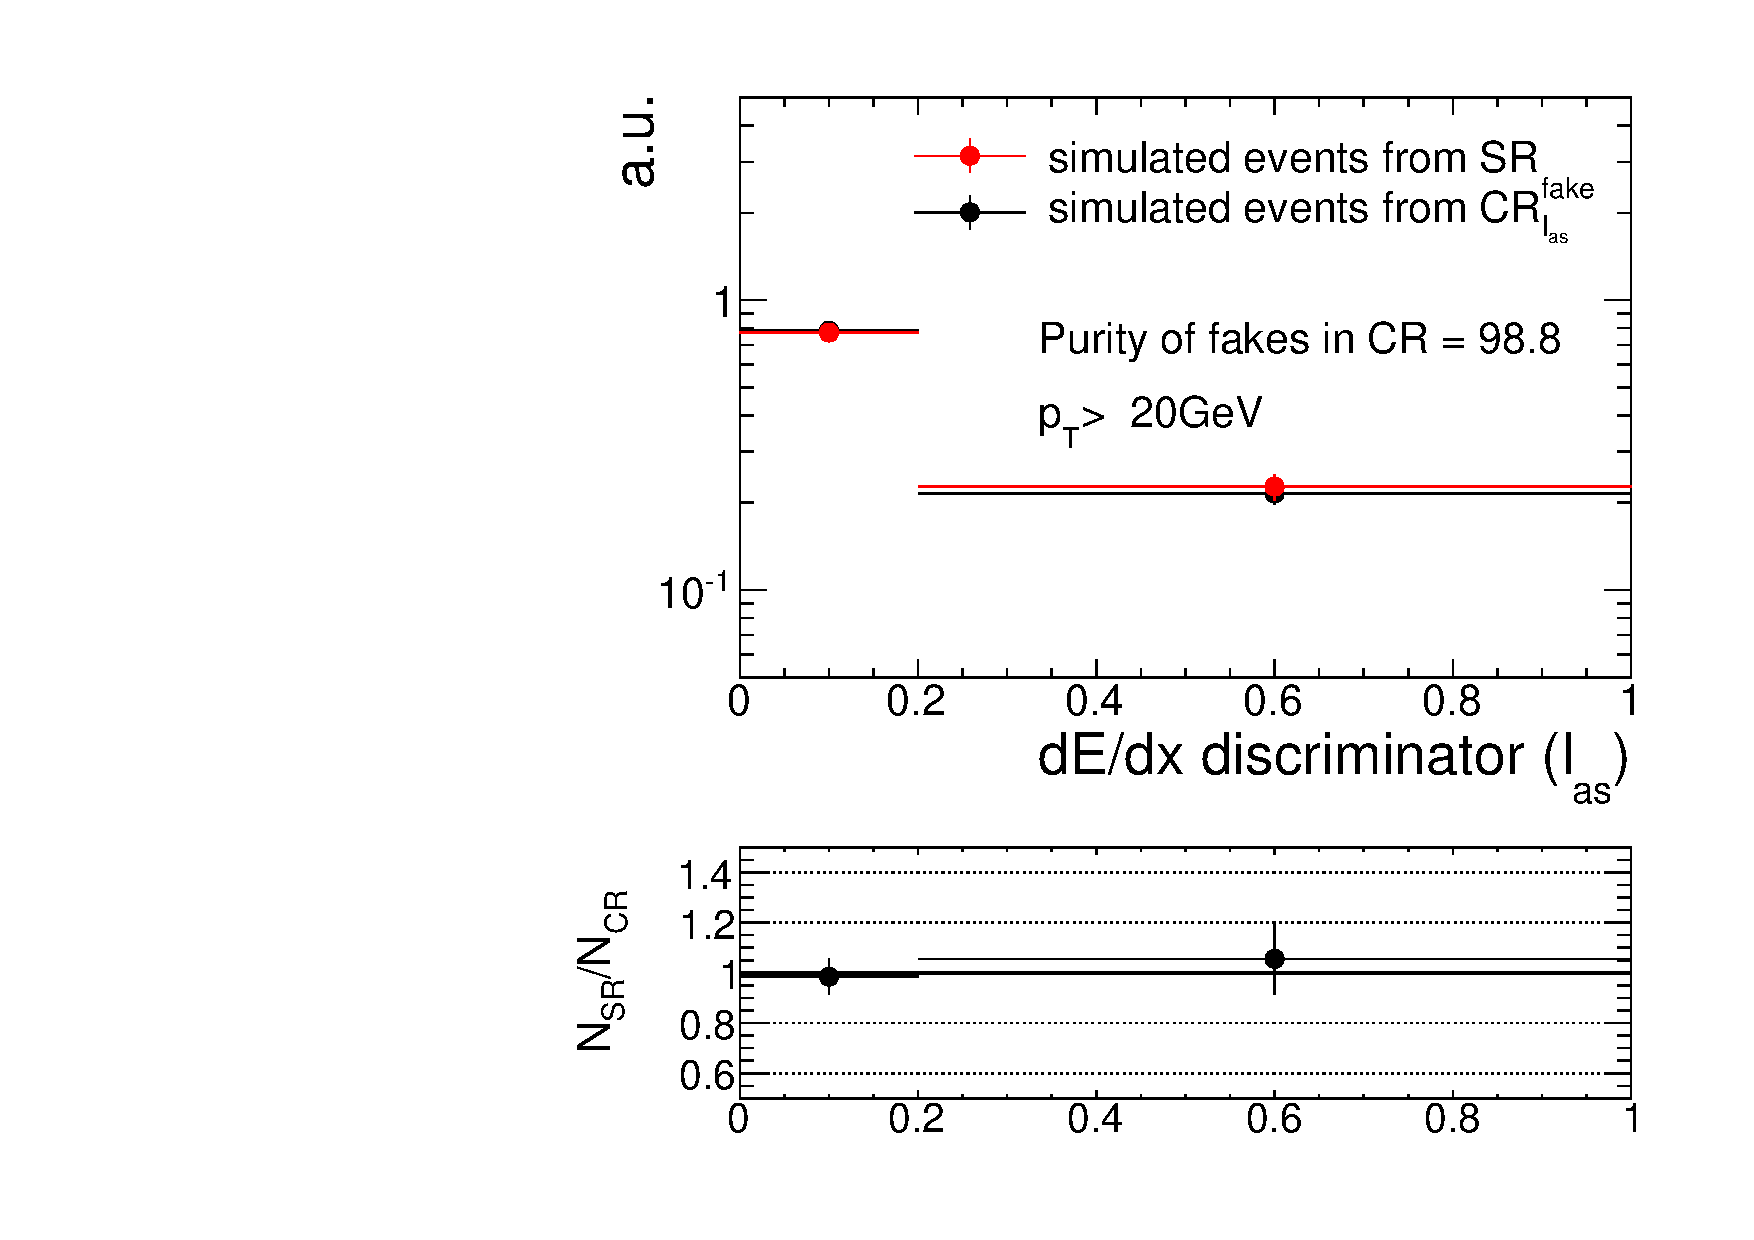
\includegraphics[width=0.49\textwidth]{figures/analysis/Background/hASmi_SRbinning_fakes_ECalaoLe5_trackPtGt20_MC_CR_MC_SR.pdf}
    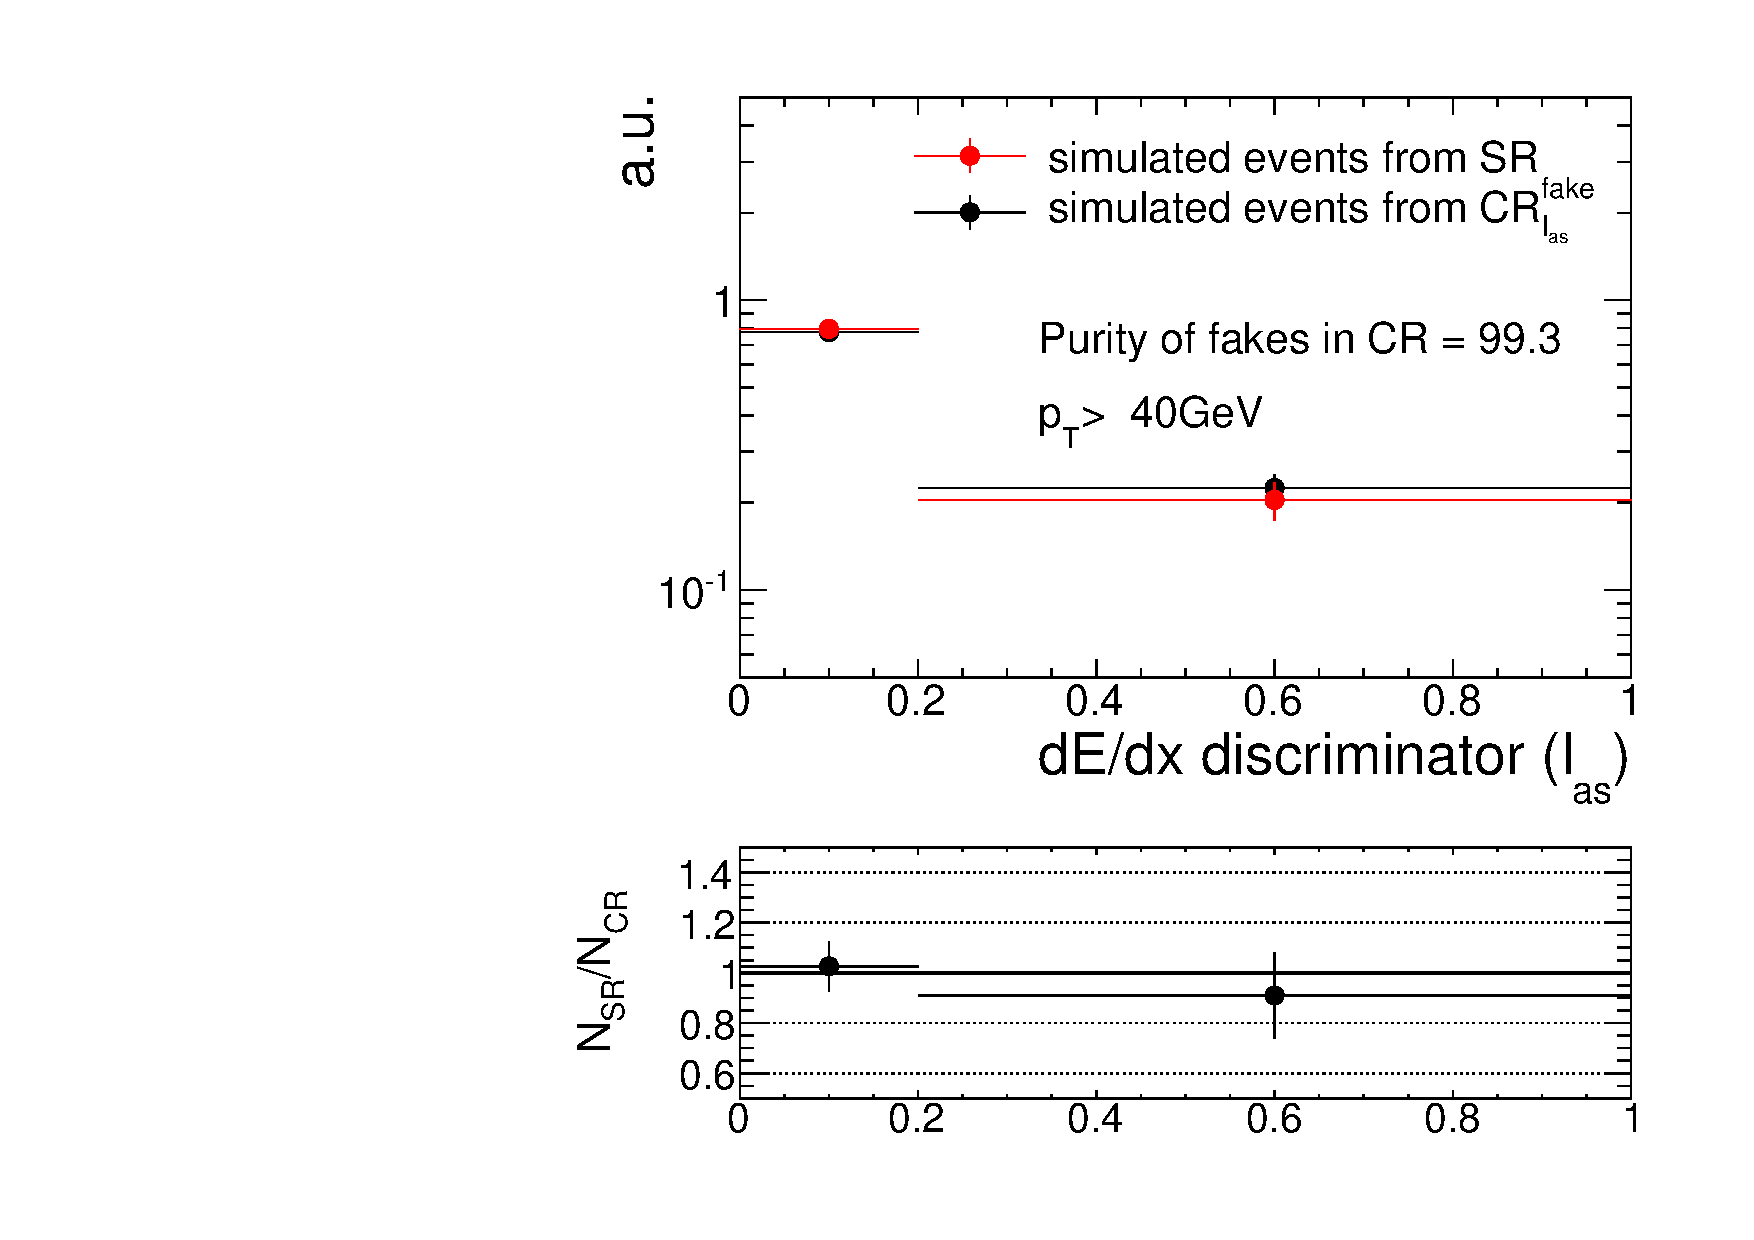
\includegraphics[width=0.49\textwidth]{figures/analysis/Background/hASmi_SRbinning_fakes_ECalaoLe5_trackPtGt40_MC_CR_MC_SR.pdf}
  \end{tabular}
  \caption{Underlying histograms to estimate the fake \ias systematic uncertainty. 
           Normalised distributions of the \ias shape of fake tracks in the signal and control region of simulated \WJets events with a \pt selection of 20\gev (left) and a 40\gev (right).}
  \label{fig:FakeIasUnc}
\end{figure}

%%%%%%%%%%%%%%%%%%%%%%%%%%%%%%%%%%%%%%%%%%%%%%%%%%%%%%%%%%%%%%%%%%%%%%%%%%%%%%%%%%%%%%%%%%%%%%%%%%%%%%%%%%%%%%%%%%%%%%%%%%%%%%%%%%%%%%%%%%%%%%%%%%%%%%%%%%%%%%%%%%%%%%%
\subsection{Uncertainty on the leptonic scale factor}
\label{sec:LeptonScaleUncertainty}

The leptonic scale factor \leptonscalefactor is estimated on simulated \WJets events.
The corresponding systematic uncertainty that addresses the use of information from simulation is derived by a ``tag-and-probe'' method conducted on real data and simulated events.

For this method a selection of \Zlep events is done with one ``tagged'' well reconstructed lepton and one ``probed'' candidate track.
To ensure a selection of \Zlep events, a selection on the invariant mass of  the reconstructed lepton and the candidate track is applied with $80\gev<M_{\text{inv}}\left( \text{lepton}, \text{cand. trk}  \right)<100\gev$ for muons and electrons.
For taus, a muon from a $\tau\rightarrow\mu\nu\nu$ decay is selected with $40\gev<M_{\text{inv}}\left( \mu, \text{cand. trk}  \right)<75\gev$ and $m_T\left(\mu,\met\right)<40\gev$~\cite{bib:CMS:DT_Thesis,bib:CMS:DT_8TeV_AN}.
Furthermore, the candidate track and the lepton are required to be opposite in charge.
In order to reduce the contamination of fakes in the ``tag-and-probe'' samples an additional selection on the number of hits of $\nhits>5$ is required.

The ``tag-and-probe'' selection is done for each lepton type separately.
In order to determine the leptonic scale factors, the number of events is once estimated for the candidate track selection including the corresponding lepton veto which gives the a number of events in the ``tag-and-probe'' signal region $N_{SR}^{\text{T\&P}}$, and once inverting the lepton veto selection requirement which gives the the number of events in the ``tag-and-probe'' lepton inverted control region $N_{\text{CR, lepton veto inverted}}^{\text{T\&P}}$.
As for the determination of the tau and electron scale factor with simulated \WJets events, no requirement on the calorimeter isolation is applied in the lepton veto inverted control region for taus and electrons.
This leads to the following expression of the lepton scale factor for muons
\begin{equation*}
\rho^{\mu} = \frac{N_{\text{SR}}^{\text{T\&P}\mu}}{N_{\text{CR, }\mu\text{ veto inverted}}^{\text{T\&P}}}.
\end{equation*}
and for electrons and taus 
\begin{equation*}
\rho^{e,\tau} = \frac{N_{\text{SR}}^{\text{T\&P}e,\tau}}{N_{\text{CR, }e,\tau \text{ veto inverted}}^{\text{T\&P}}}.
\end{equation*}

%As candidate tracks originating from leptons anyway have almost ever \nhits grater five, this does not bias the result (see Fig.~\ref{}).
The selection requirements for the three tag-and-probe samples are listed in Tables~\ref{tab:MuonTagAndProbeSample},~\ref{tab:TauTagAndProbeSample} and~\ref{tab:ElectronTagAndProbeSample} in Appendix~\ref{app:TagAndProbeRequirements}.

The leptonic scale factors are calculated using simulated \Zlep events and real data from the single-muon and single-electron samples listed in Table~\ref{tab:ElectronMuonCRDatasets}.
The 1-sigma difference of the ratio $\rho^{\text{lep}_i}_{\text{MC}}$/$\rho^{\text{lep}_i}_{\text{Data}}$ from unity is taken as systematic uncertainty. 
This results for the signal candidate selection in an uncertainty of 69\% for the electron, 39\% for the muon and 79 \% for the tau scale factor.

%%%%%%%%%%%%%%%%%%%%%%%%%%%%%%%%%%%%%%%%%%%%%%%%%%%%%%%%%%%%%%%%%%%%%%%%%%%%%%%%%%%%%%%%%%%%%%%%%%%%%%%%%%%%%%%%%%%%%%%%%%%%%%%%%%%%%%%%%%%%%%%%%%%%%%%%%%%%%%%%%%%%%%%
\subsection{Uncertainty on the leptonic dE/dx shape}
\label{sec:LeptonIasUncertainty}

The uncertainty on lepton \ias shape is estimated by a comparison of the \ias shape in data and simulation in the lepton veto inverted control region.
Figure~\ref{fig:LeptonIasUnc} shows the leptonic \ias distributions for all three lepton types in the lepton veto inverted control region in data and simulation.
The 1-sigma difference of the ratio of the number of events in the control region in data and simulation from 1 is taken as systematic uncertainty.
This leads for example to uncertainties between $37\%-81\%$ for the signal candidate selection plus a selection requirement of $\ias>0.2$.
\begin{figure}[!h]
  \centering 
  \begin{tabular}{c}
    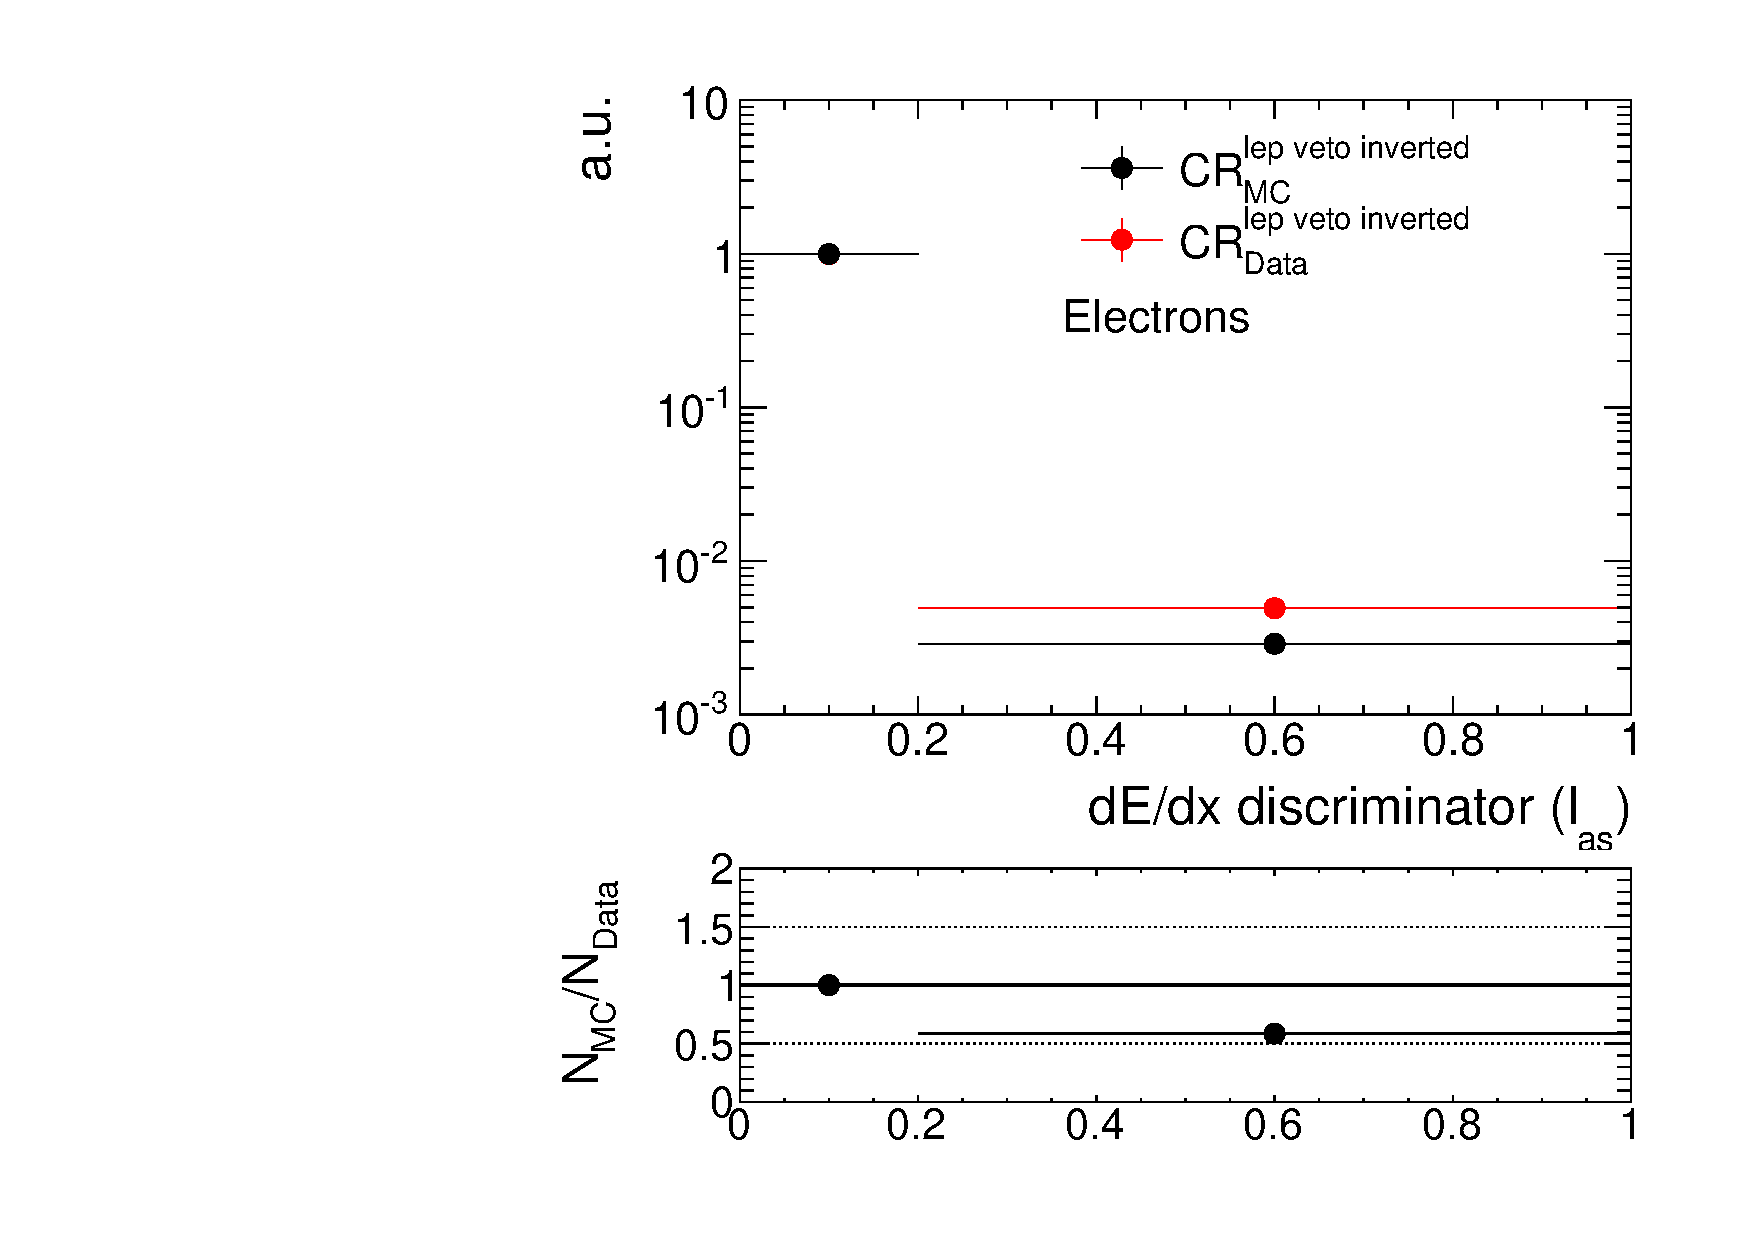
\includegraphics[width=0.33\textwidth]{figures/analysis/Background/hASmi_SRbinning_Electrons_MCCR_DataCR.pdf}
    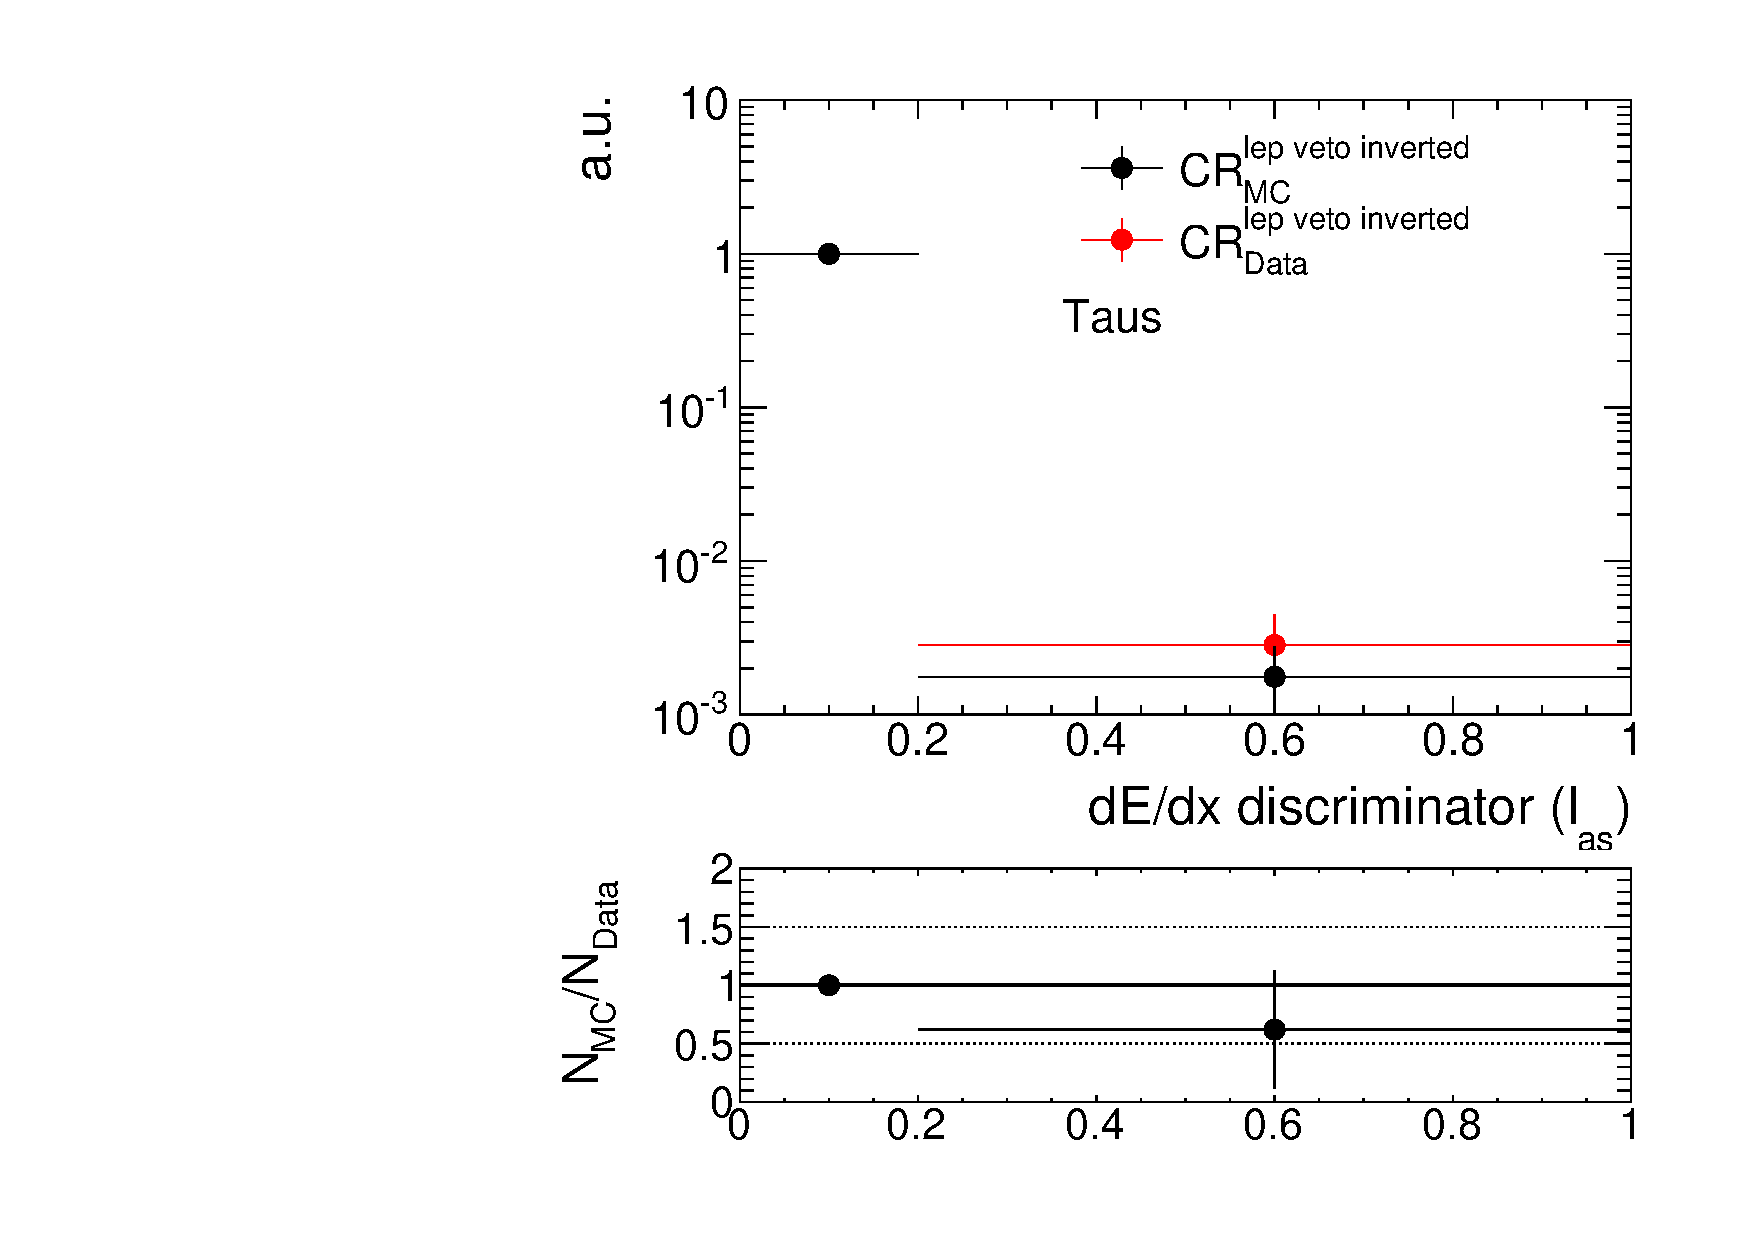
\includegraphics[width=0.33\textwidth]{figures/analysis/Background/hASmi_SRbinning_Taus_MCCR_DataCR.pdf}
    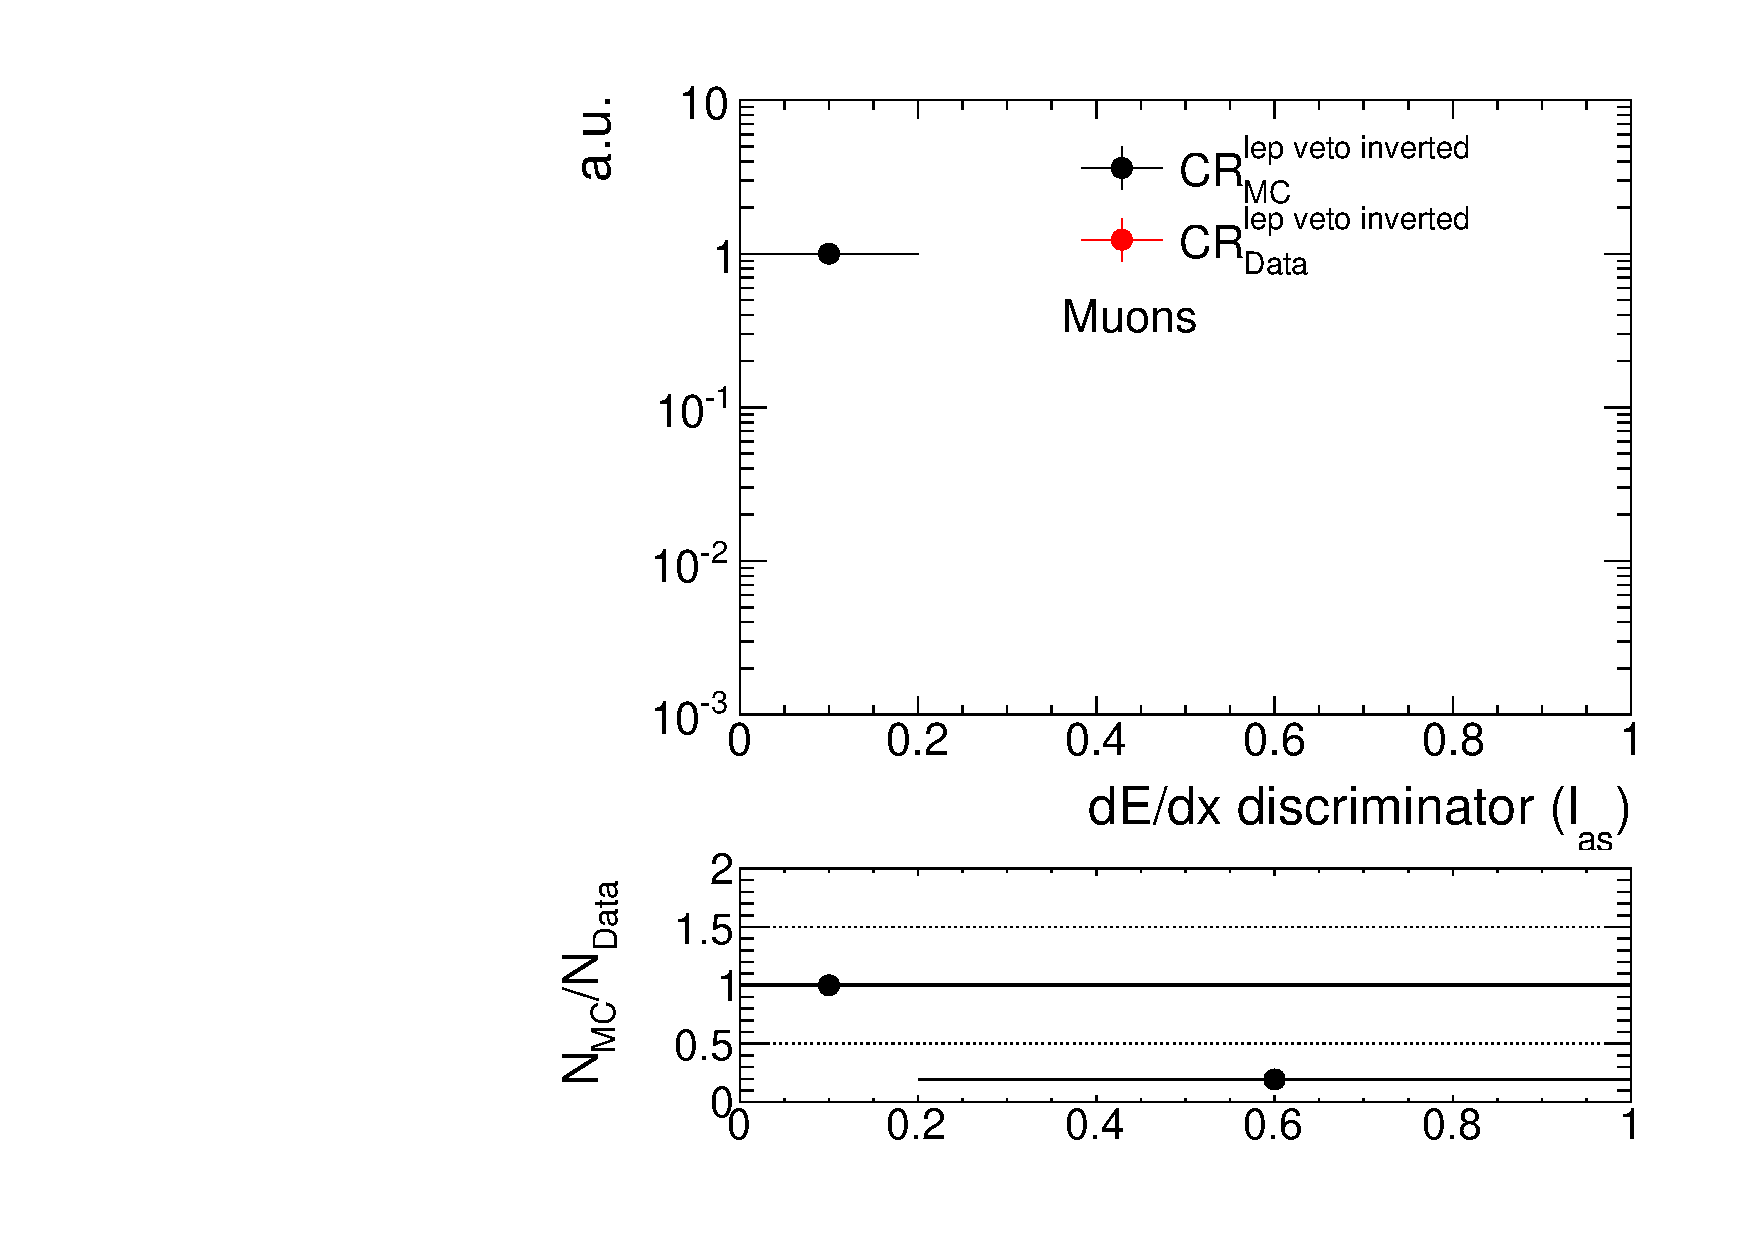
\includegraphics[width=0.33\textwidth]{figures/analysis/Background/hASmi_SRbinning_Muons_MCCR_DataCR.pdf}
  \end{tabular}
  \caption{Underlying histograms to estimate the leptonic \ias systematic uncertainty. Normalised distributions of the lepton \ias distributions in the lepton veto inverted control region for data (red) and simulation (black) for all three lepton types. The event-based selection requirements and the calorimeter isolation requirement are removed to enhance the statistical precision.}
  \label{fig:LeptonIasUnc}
\end{figure}

%%%%%%%%%%%%%%%%%%%%%%%%%%%%%%%%%%%%%%%%%%%%%%%%%%%%%%%%%%%%%%%%%%%%%%%%%%%%%%%%%%%%%%%%%%%%%%%%%%%%%%%%%%%%%%%%%%%%%%%%%%%%%%%%%%%%%%%%%%%%%%%%%%%%%%%%%%%%%%%%%%%%%%%
%%%%%%%%%%%%%%%%%%%%%%%%%%%%%%%%%%%%%%%%%%%%%%%%%%%%%%%%%%%%%%%%%%%%%%%%%%%%%%%%%%%%%%%%%%%%%%%%%%%%%%%%%%%%%%%%%%%%%%%%%%%%%%%%%%%%%%%%%%%%%%%%%%%%%%%%%%%%%%%%%%%%%%%
